\documentclass[french]{article}


\usepackage[utf8]{inputenc} % encode en UTF8

\usepackage[T1]{fontenc}





\usepackage[top=2cm, bottom=2cm, left=3cm, right=3cm]{geometry}
\usepackage{graphicx}
\usepackage{caption}
\usepackage{subcaption}
\usepackage{float}
\graphicspath{ {./photo/} }

%Belles fraction de fration \cfrac
\usepackage{amsmath}

\usepackage{tikz}
\usepackage{circuitikz}




\newcommand{\HRule}{\rule{\linewidth}{0.5mm}} % Epaisseur des lignes horizontales

\pagestyle{empty}
\newcommand{\myTitle[1]}{
\begin{minipage}{.47\textwidth}
\centering
\begin{flushleft}

\includegraphics[width=0.75\textwidth]{./photo/nantes_universite_logo.png}
\end{flushleft}
\end{minipage}
\begin{minipage}{.47\textwidth}
\centering
\begin{flushright}
\hspace*{1cm} 
\includegraphics[width=0.85\textwidth]{./photo/logo_polytech_nantes}
\end{flushright}
\end{minipage}~\\[1.5cm]

\begin{center}
\vspace*{\stretch{0.3}}
\end{center}

\begin{center}
  \Large
  \vspace*{\stretch{1}}
  \HRule \\[0.2cm]
  \begin{center}
    \huge
    \textbf{#1}\\ %Titre
  \end{center}
  %\textbf{\\ Projet Transversal}\\ %matière
  \HRule \\[1.5cm]
  
%  \vspace*{\stretch{5}}
%  
%  \small
%  \noindent Rédigé par \\
%  \vspace*{\stretch{0.2}}
%  \large
%  \noindent \Redac\\
%  \vspace*{\stretch{0.5}}
 
\end{center}

\vspace*{\stretch{2}}

\begin{center}\large
	\textsc{École Polytech de Nantes}\\
	\textsc{Département Électronique et Technologie du Numérique}
\end{center}

\vspace*{\stretch{5}}

\begin{center}
	\begin{minipage}{0.4\textwidth}
		\begin{flushleft} \large
        	\noindent Rédigé par\\ %\Redac
			Victor DUFRENE \\
			Mathis BRIARD\\
			Louison GOUY\\
			Yujie HUANG
		\end{flushleft}
	\end{minipage}
	\begin{minipage}{0.4\textwidth}
		\begin{flushright}\large
			Professeur encadrant : \\Yann MAHE\\ Anne CHOUSSEAUD\\
						
		\end{flushright}
	\end{minipage}
\end{center}
}

\begin{document}
\myTitle[Rapport de mini-projet \\ - Électronique Hautes Fréquences - ]
\newpage

\textbf{Il faudra pas oublier de rajouter une table des figures et matières}

\section{Résumé}
\textbf{Resume le mini-projet}

\section{Introduction}
\subsection{Contextualisation}
\textbf{Parler de la limite entre BF et HF (longueur du circuit plus négligeable devant la longueur d'onde des signaux mis en jeu)\\
parler des applications de l'electronique haute frequence}
\subsection{Objectifs du mini-projet}
\textbf{developpement connaissance en electronique haute frequence\\
prise en main de logiciel de conception et de simulations (ADS)}

\newpage

\section{Étude et caractérisation de la technologie micro-ruban}

\subsection{Avant-propos}

L'électronique des hautes-fréquences consiste en la propagation de signaux à fréquences élevées, et de longueurs d'ondes proches des dimensions du circuit, au travers d'une ligne de transmission. Les lignes de transmissions se déclinent sous diverses familles comme les câbles coaxiaux, les lignes bifilaires, les guides d'ondes ou encore les lignes micro-rubans. Comme le schématise la figure (\ref{fig:modele_microstrip}), une ligne micro-ruban (\textit{microstrip line}) est composée d'un conducteur planaire séparé d'un plan de masse par une couche diélectrique appelée substrat. Une telle technologie a été développée par les laboratoires ITT (\textit{International Telephone and Telegraph}) dans les années 1952. Simple de fabrication et coût bas au regard des autres technologies, la ligne micro-ruban permet la conception de nombreuses fonctions d'électroniques comme le filtrage ou l'amplification.

\begin{figure}[H]
	\centering
	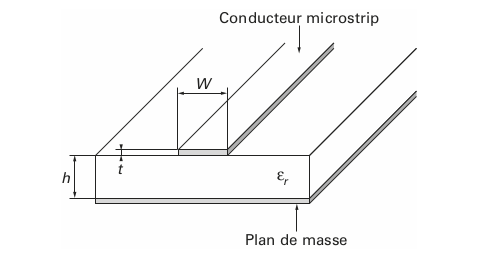
\includegraphics[width=0.8\linewidth]{ressources/modele_microstrip.png}
	\caption{Modèle d'une ligne micro-ruban}
	\label{fig:modele_microstrip}
\end{figure}

Il s'agit dans cette partie de réaliser des caractérisations de lignes, c'est-à-dire la détermination de paramètres d'une ligne micro-ruban. Les lignes à caractériser sont disponibles en laboratoire et sont de l'ordre de quatre, une ligne verre téflon large, verre téflon fin, verre epoxy FR4 large et verre epoxy FR4 fin. Des photographies de ces plaques sont présentes en annexe. Le tableau précisant les dimensions de ces quatre lignes est donné ci-dessous. La caractérisation aura pour finalité l'obtention des paramètres de la ligne telle que la constante diélectrique $\varepsilon_r$ du matériau ainsi que la tangente de perte $\mbox{tan}(\delta)$. Ces paramètres serviront par la suite de valeurs de référence pour la conception de filtres ou d'amplificateurs en technologie micro-ruban. Il s'agit alors de réaliser des mesures à l'aide d'un analyseur de réseau, VNA (\textit{Vector Network Analyzer)}, pour en extraire les valeurs de la matrice $S$. Ces mesures expérimentales constituent la base de la caractérisation. Un modèle théorique de caractérisation de lignes vient se superposer à cette base. Il s'agira alors de faire varier les divers paramètres du modèle afin de faire coïncider celui-ci avec les mesures expérimentales. À ce moment là, les paramètres du modèle correspondent aux paramètres de la ligne et la caractérisation est réussie.


\begin{table}[H]
	\centering
	\begin{tabular}{|c|c|c|c|c|}
		\hline
		Matériaux & Impédance caractéristique & hauteur $h$ & largeur $W$ & longueur $L$\\
		\hline
		Verre téflon large & $Z_C < 50 \Omega$ & 1.58 & 7.87 & 74.82 \\
		\hline
		Verre téflon fin & $Z_C > 50 \Omega$ & 1.58 & 0.469 & 74.978\\
		\hline
		Verre epoxy FR4 large & $Z_C < 50 \Omega$ & 1.50 & 7.928 & 100.037\\
		\hline
		Verre epoxy FR4 fin & $Z_C > 50 \Omega$ & 1.50 & 0.46 & 100.44\\
		\hline
	\end{tabular}
	\caption{Tableau présentant les paramètres géométriques (exprimés en mm) des différentes lignes à caractériser}
\end{table}

\newpage

\subsection{Présentation du modèle théorique de caractérisation large bande de lignes}

Cette section est consacrée à la présentation d'une structure modélisant le comportement d'une ligne de caractérisation. Un tel modèle possède divers paramètres dont il est nécessaire de déterminer leur valeurs offrant la meilleure superposition avec les courbes expérimentales. Un schéma de ce modèle est présenté ci-dessous. Celui-ci comporte aux extrémités deux terminaux TERM 1 et TERM 2 qui représentent les câbles coaxiaux SMA (\textit{Subminiature version A}) de 50 $\Omega$ du VNA. Les composants MLIN 1 (\textit{Microstrip line 1}), MLIN 2 et 3 sont des lignes micro-rubans de largeur et longueur respectives $W_{acc1}$ et $L_{acc1}$, $W$ et $L$ et $W_{acc2}$ et $L_{acc2}$. MLIN 1 et MLIN 3 modélisent les lignes d'accès et MLIN 2 correspond à la ligne micro-ruban à caractériser. Un tableau ci-dessous précise les différents paramètres.

\begin{table}[H]
	\centering
	\begin{tabular}{|c|c|c|c|c|c|c|}
		\hline
		Matériaux & $W_{acc1}$ & $L_{acc1}$ & $W_{acc2}$ & $L_{acc2}$ & $W$ & $L$\\
		\hline
		Verre téflon large & 4.278 & 5.345 & 4.225 & 5.349 & 7.87 & 74.82 \\
		\hline
		Verre téflon fin & 4.397 & 5.385 & 4.302 & 4.925 & 0.469 & 74.978\\
		\hline
		Verre epoxy FR4 large & 2.918 & 10.031 & 2.944 & 10.063 & 7.928 & 100.037\\
		\hline
		Verre epoxy FR4 fin & 2.862 & 9.982 & 2.914 & 9.948 & 0.46 & 100.44\\
		\hline
	\end{tabular}
	\caption{Tableau présentant les paramètres géométriques (exprimés en mm) des différents MLIN}
\end{table}


\begin{figure}[H]
	\centering
	\begin{circuitikz}[scale=0.90]
	\draw (1,-0.5) to (1,0.5);
	\draw (1,0.5) to (-1,0.5);
	\draw (-1,0.5) to (-1,-0.5);
	\draw (-1,-0.5) to (1,-0.5);
	\draw (1,0) to (1.5,0);
	\draw (-1,0) to (-1.5,0);
	\draw (-1.5,-0.5) to (-1.5,0.5);
	\draw (1.5,-0.5) to (1.5,0.5);
	\draw (1.5,-0.5) to (2,-0.5);
	\draw (1.5,0.5) to (2,0.5);
	\draw (2,0.5) to (2,0.25);
	\draw (2,-0.5) to (2,-0.25);
	\draw (-1.5,0.5) to (-2,0.5);
	\draw (-1.5,-0.5) to (-2,-0.5);
	\draw (-2,-0.5) to (-2,-0.25);
	\draw (-2,0.5) to (-2,0.25);
	\draw (-2,0.25) to (-2.5,0.25);
	\draw (-2.5,0.25) to (-2.5,-0.25);
	\draw (-2.5,-0.25) to (-2,-0.25);
	\draw (2,0.25) to (2.5,0.25);
	\draw (2.5,0.25) to (2.5,-0.25);
	\draw (2.5,-0.25) to (2,-0.25);
	\draw (2.5,0) to (3,0);
	\draw (-2.5,0) to (-3,0);
	\draw (-3,0.25) to (-3,-0.25) to (-4,-0.25) to (-4,0.25) to (-3,0.25);
	\draw (3,0.25) to (3,-0.25) to (4,-0.25) to (4,0.25) to (3,0.25);
	\draw (4,0) to (4.5,0);
	\draw (-4,0) to (-4.5,0);
	\ctikzset{inductors/scale=0.9,inductor=american}
	\draw (4.5,0) to [L=$L_{dis}$] (5.5,0);
	\draw (5.5,0) to (7.5,0);
	\draw (6,0) to (6,-0.5);
	\draw (-4.5,0) to [L, l_=$L_{dis}$, mirror] (-5.5,0);
	\draw (-5.5,0) to (-7.5,0);
	\draw (-6,0) to (-6,-0.5);
	%\ctikzset{polar capacitor, C,l=$C_{dis}$}
	\draw (-6,-0.5) to [capacitor, C ,l=$C_{dis}$] (-6,-2) node[ground]{};
	\draw (6,-0.5) to [capacitor, C ,l_=$C_{dis}$] (6,-2) node[ground]{};
	\draw (-7.5,0) to (-7.5,-0.25) to [R] (-7.5,-2) node[ground]{};
	\draw (-8,-0.25) to (-7,-0.25) to (-7,-2) to (-8,-2) to (-8,-0.25);
	\draw (7.5,0) to (7.5,-0.25) to [R] (7.5,-2) node[ground]{};
	\draw (8,-0.25) to (7,-0.25) to (7,-2) to (8,-2) to (8,-0.25);
	\node at (0,0.75) {MLIN2};
	\node at (-3.5,0.5) {MLIN1};
	\node at (3.5,0.5) {MLIN3};
	\node at (-2,-0.75) {MSTEP1};
	\node at (2,-0.75) {MSTEP2};
	\node at (-7.5,0.25) {TERM 1};
	\node at (7.5,0.25) {TERM 2};
\end{circuitikz}
	\caption{Schéma représentatif du modèle de caractérisation de lignes}
	\label{fig:schema_modele_caract}
\end{figure}

Les résonateurs $L_{dis}C_{dis}$ ainsi que les composants MSTEP 1 et MSTEP 2 sont utilisés dans ce modèle pour prendre en compte des phénomènes de discontinuités. Les largeurs entre les lignes MLIN 1, MLIN 2 et MLIN 3 sont différentes et mènent à une déformation des champs électromagnétiques à l'interface entre ces lignes. Les composants MSTEP 1 et MSTEP 2 modélisent cette interface et ajoute cette discontinuité de largeur au modèle\footnote{Un tel phénomène de discontinuité peut être utile et mis à profit du concepteur. En effet, ces changements brutes de largeur de lignes permettent de réaliser des transformateurs d'impédances.}. En ce qui concerne les résonateurs $L_{dis}C_{dis}$, ces cellules prennent en compte la modification de la distribution du champ électromagnétique à l'interface entre le câble SMA et la plaque. En effet, le champ électromagnétique passe d'une distribution cylindrique à une distribution planaire.


\begin{figure}[H]
	\centering
	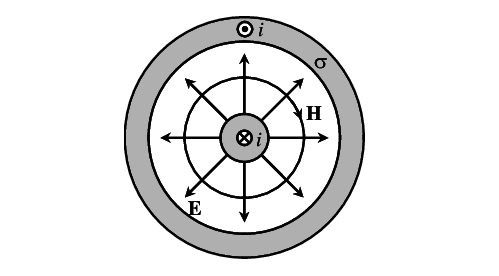
\includegraphics[scale=0.8]{ressources/electromagnetic_distribution_coaxial.png}
	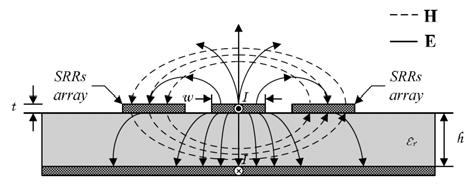
\includegraphics[scale=0.5]{ressources/electromagnetic_distribution_microstrip.png}
	\caption{Schéma de coupe normal à la direction de propagation représentant les distributions du champ électromagnétique dans un câble coaxial (à gauche) et dans une ligne micro-ruban (à droite)}
	\label{fig:schema_distribution_EOM}
\end{figure}

\newpage

Dans le cas de la ligne micro-ruban, il est possible de remarquer des effets de bord du champ électrique. Ces effets de bord sont également présents selon la direction de propagation (non visible sur la figure \ref{fig:schema_distribution_EOM}). Le mode de propagation n'est donc pas un mode TEM car une telle distribution présente des composantes du champ $\overrightarrow{E}$ selon l'axe de propagation, à cause des effets de bord. Cependant, il est possible de poser l'hypothèse d'un mode quasi-TEM à la condition d'être loin des extrémités de la ligne pour éviter les fuites du champ $\overrightarrow{E}$. En effet avec cette condition, sur une tranche infinitésimale le mode de propagation est considéré comme un mode TEM. Dans la suite du rapport, le mode de propagation utilisé sera un mode quasi-TEM. Afin d'approximer la propagation à un mode quasi-TEM, il est aussi nécessaire de travailler non pas avec la constante diélectrique $\varepsilon_r$ mais avec la constante $\varepsilon_{reff}$. Cela sera abordé plus tard dans le rapport.

\subsection{Caractérisation large bande des lignes micro-rubans sous ADS}

Il s'agit dans cette section de réaliser les quatre caractérisations en s'appuyant sur le modèle théorique décrit précédemment. Sur l'ensemble des paramètres à déterminer, il a été possible de fixer les paramètres géométriques par mesures directes sur les plaques. Le nombre d'inconnues est grandement réduit et les valeurs à fixer sont la constante diélectrique $\varepsilon_r$, la tangente de perte $\mbox{tan}(\delta)$ ainsi que l'inductance $L_{dis}$ et la capacité $C_{dis}$ des cellules résonatrices.\\
Le logiciel de conception et de simulation ADS offre un ensemble d'outils utile à la caractérisation des divers substrats. La figure ci-dessous représente le modèle théorique transposé sur ADS. Le composant \texttt{MSub} est utilisé pour donner les caractéristiques géométriques et électriques de la ligne micro-ruban. \texttt{H} représente la hauteur $h$ de la figure (\ref{fig:modele_microstrip}), c'est-à-dire la distance entre le plan de masse et la ligne micro-ruban. \texttt{Er} et \texttt{Mur} sont respectivement la permittivité diélectrique $\varepsilon_r$ et la perméabilité magnétique $\mu_r$. Le paramètre \texttt{Cond} correspond à la conductivité du matériaux utilisé. Dans le cas du cuivre (Cu), sa conductivité $\sigma$ est de l'ordre de $5,87.10^{7}$ S/m. \texttt{Hu} représente la hauteur de la cage dans le cas d'une conception de ligne micro-ruban avec blindage, \texttt{T} est le paramètre $t$ de la figure (\ref{fig:modele_microstrip}), c'est-à-dire la hauteur de la couche de métallisation. Dans les technologies de photolithographie utilisées pour les plaques en laboratoire, en prenant en compte le phénomène de sous-gravure il faut espérer obtenir une précision de 17 ou 35 $\mu m$. Le paramètre \texttt{Rough} représente la rugosité du métal. Un tel paramètre permet de prendre en compte de l'état de surface, parfois inhomogène, du matériaux.\\
Le paramètre \texttt{TanD} correspond à la tangente de perte $\mbox{tan}(\delta)$. Cette grandeur est définie comme le rapport de la partie imaginaire sur la partie réelle de la constante diélectrique $\varepsilon_r$. En effet pour un matériau réel, des pertes diélectriques peuvent apparaître au sein de celui-ci. Cet aspect de perte est formalisé mathématiquement par une partie imaginaire négative. Ainsi la permittivité diélectrique s'écrit :

\begin{equation}
	\varepsilon_r=\varepsilon'-j\varepsilon''=\varepsilon'(1-j\frac{\varepsilon''}{\varepsilon'}) \mbox{ avec } \mbox{tan}(\delta)=\frac{\varepsilon''}{\varepsilon'}
\end{equation}

\begin{figure}[H]
	\centering
	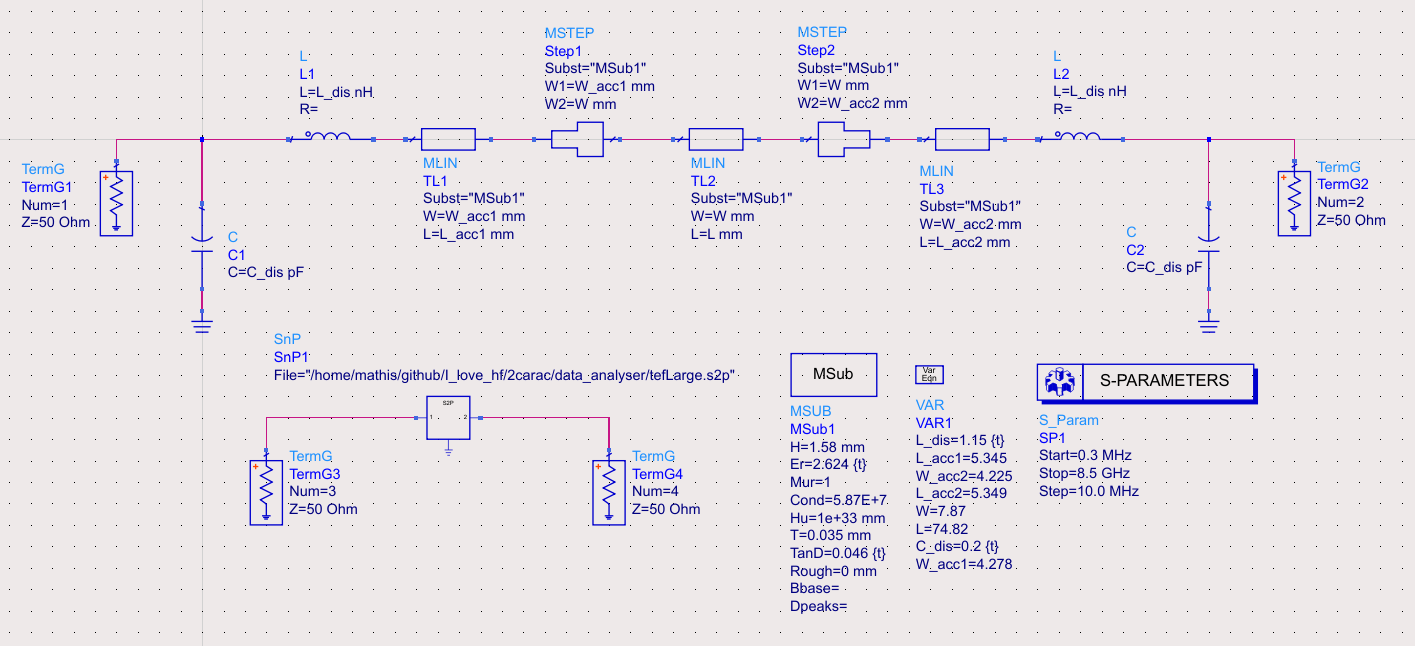
\includegraphics[scale=0.29]{../2carac/caract_large_bande/modele_ADS.png}
	\caption{Structure du modèle de caractérisation sur ADS}
	\label{fig:modele_caract_ADS}
\end{figure}

\newpage

Suite à l'implémentation du modèle théorique de caractérisation de ligne sur ADS, les simulations sont réalisées en respectant les dimensions de chaque plaque. Les quatre cas sont donnés dans la figure ci-dessous présentant l'évolution du paramètre $S_{11}$, le coefficient de réflexion en entrée, en fonction de la fréquence $f$.

\begin{figure}[H]
	\centering
	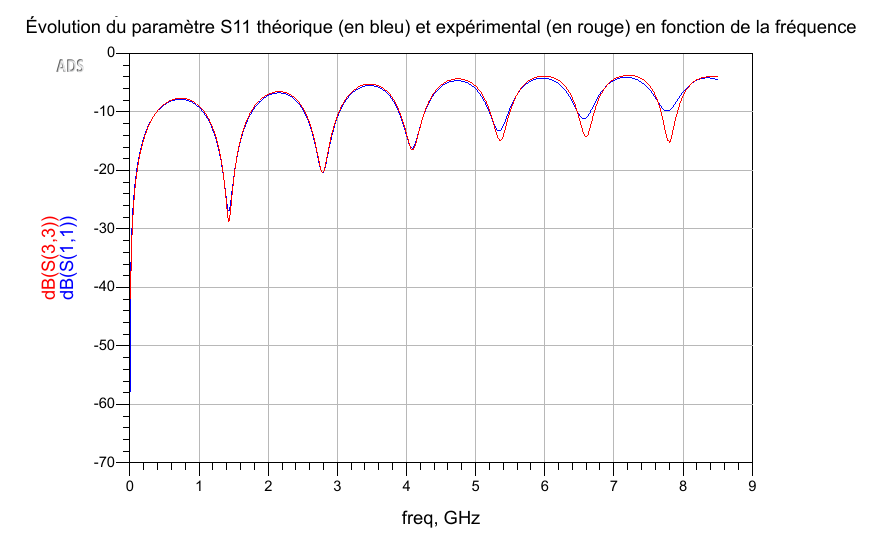
\includegraphics[scale=0.24]{../2carac/caract_large_bande/caract_large_bande_teflarge.png}
	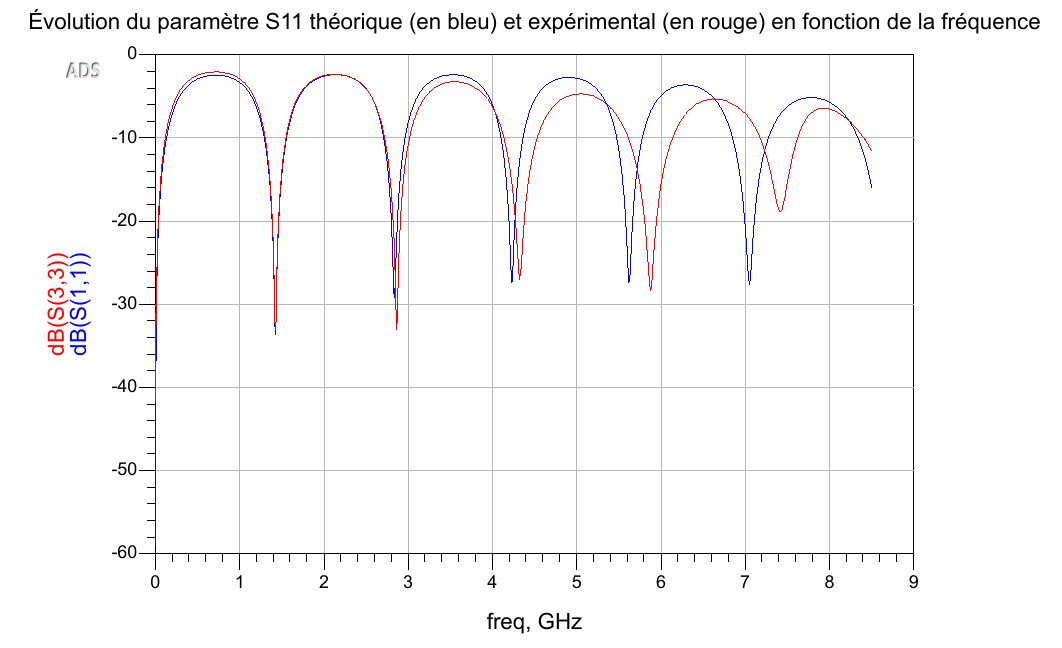
\includegraphics[scale=0.20]{../2carac/caract_large_bande/caract_large_bande_teffin.png}\\
	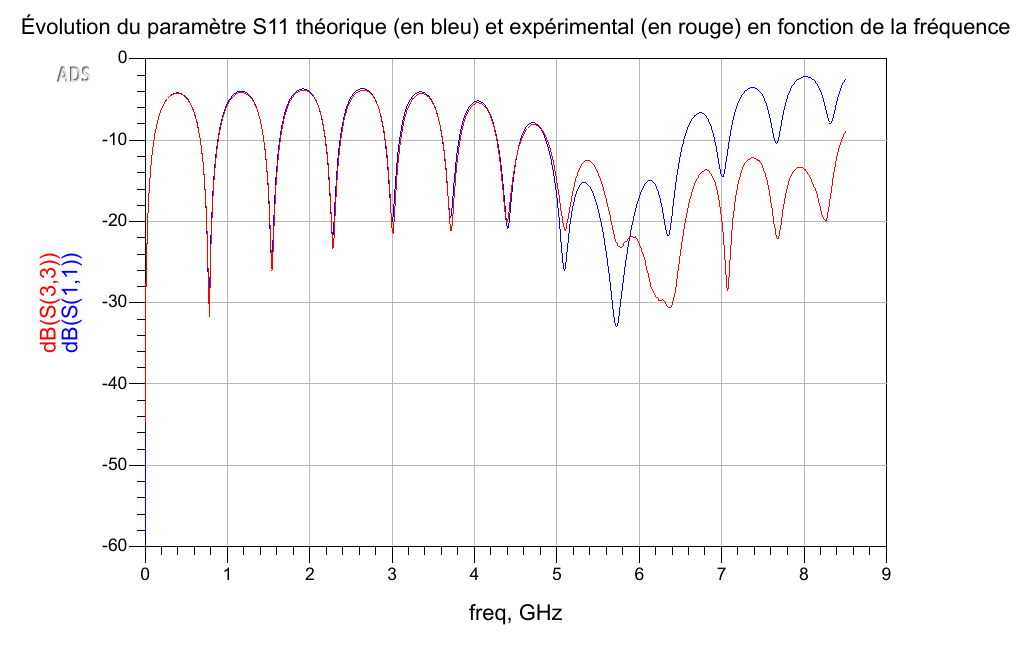
\includegraphics[scale=0.20]{../2carac/caract_large_bande/caract_large_bande_epoxylarge.png}
	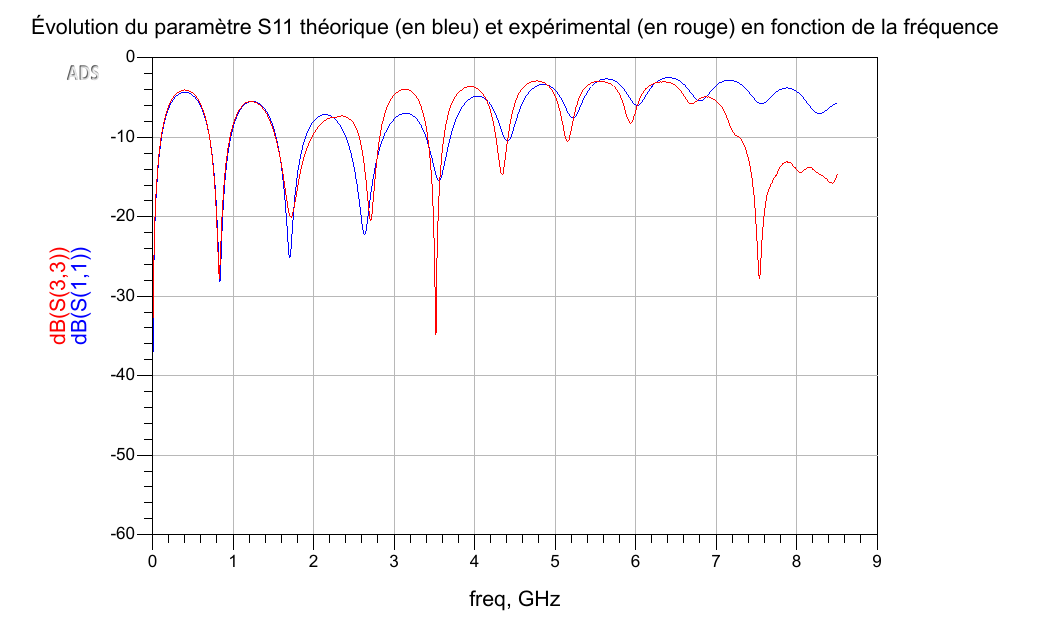
\includegraphics[scale=0.21]{../2carac/caract_large_bande/caract_large_bande_epoxyfin.png}
	\caption{Graphique représentant les résultats de caractérisation large bande pour le téflon large (en haut à gauche), téflon fin (en haut à droite), epoxy large (en bas à gauche) et epoxy fin (en bas à droite)}
	\label{fig:caracterisations}
\end{figure}

La superposition des résultats expérimentaux (courbe rouge) avec le résultat du modèle de caractérisation (courbe bleu) est effectué à l'aide du mode \texttt{tuning} d'ADS. Un tel mode laisse la main au concepteur pour modifier en temps-réel les paramètres qu'il souhaite, dans le cas de ces caractérisations il s'agit de $\mbox{tan}(\delta)$, $L_{dis}$, $C_{dis}$ et $\varepsilon_r$. Les paramètres obtenus après réglage sont donnés dans le tableau ci-dessous. Il faut remarque que dans les lignes larges ($W$ de l'ordre de 8mm), la superposition des deux courbes s'effectue sur environ 5 ventres et nœuds tandis que pour des largeurs fines ($W$ de l'ordre de 0,5mm), la superposition est seulement sur 2 ventres et 1 nœud.

\begin{table}[H]
	\centering
	\begin{tabular}{|c|c|c|c|c|}
		\hline
		Matériaux & $\varepsilon_r$ & $\mbox{tan}(\delta)$ & $C_{dis}$ en pF & $L_{dis}$ en nH\\
		\hline
		Verre téflon large & 2.624 & 0.046 & 0.2 & 1.15\\
		\hline
		Verre téflon fin & 2.724 & 0.009 & 0.25 & 0.55\\
		\hline
		Verre epoxy FR4 large & 4.574 & 0.018 & 0.25 & 1.3\\
		\hline
		Verre epoxy FR4 fin & 4.674 & 0.048 & 0.3 & 1.45\\
		\hline
	\end{tabular}
	\caption{Résultats des paramètres de la ligne après simulation et ajustement du modèle}
\end{table}

Les paramètres sont à mettre en regard avec les données garanties par le fabricant. La fiche technique pour le verre téflon (autrement nommé PTFE, polytétrafluoroéthylène) est proposée par la société CIF (Circuit Imprimé Français). La fiche technique pour le verre epoxy FR4 est celle de LP (Laminated Plastics). Ces paramètres $\varepsilon_r$ et $\mbox{tan}(\delta)$ donnés dans le tableau ci-après ont été déterminés sous une fréquence de 1 GHz avec une hauteur de substrat de 0,062 pouce, soit 1,58 mm, qui semble être après recherche une hauteur de référence pour la documentation des fabricants.

\newpage

\begin{table}[H]
	\centering
	\begin{tabular}{|c|c|c|}
		\hline
		Matériaux (fabricant) & $\varepsilon_r$ & $\mbox{tan}(\delta)$\\
		\hline
		Verre téflon (CIF) & 2.4 à 2.65 & 0.022\\
		\hline
		Verre epoxy FR4 (LP) & 4.34 & 0.016\\
		\hline
	\end{tabular}
	\caption{Paramètres garanties par les fabricants de circuits imprimés}
\end{table}

Pour le cas de verre téflon et epoxy large ($W$ d'environ 8 mm), les valeurs obtenus sont de même ordre de grandeur que les données du fabricant. En ce qui concerne les caractérisations en largeur fine ($W$ d'environ 0,5 mm), les valeurs de la constante diélectrique ne sont pas aberrantes, cependant il y a une mauvaise évaluation de l'angle de perte $\mbox{tan}(\delta)$. Les résultats non conformes dans le cas des largeurs fines semblent être la conséquence d'une mauvaise superposition entre les deux courbes comme le montre la figure (\ref{fig:caracterisations}). Il a été cependant possible d'améliorer la caractérisation du téflon fin en modifiant le paramètre $t$, la hauteur de métallisation, à 17 $\mu m$. À l'aide de ce réglage, la constante diélectrique $\varepsilon_r$ est de 2,574, la tangente de perte $\mbox{tan}(\delta)$ est de 0,015 une inductance $L_{dis}$ de 0,9 nH et une capacité de 0,25 pF. 

\begin{figure}[H]
	\centering
	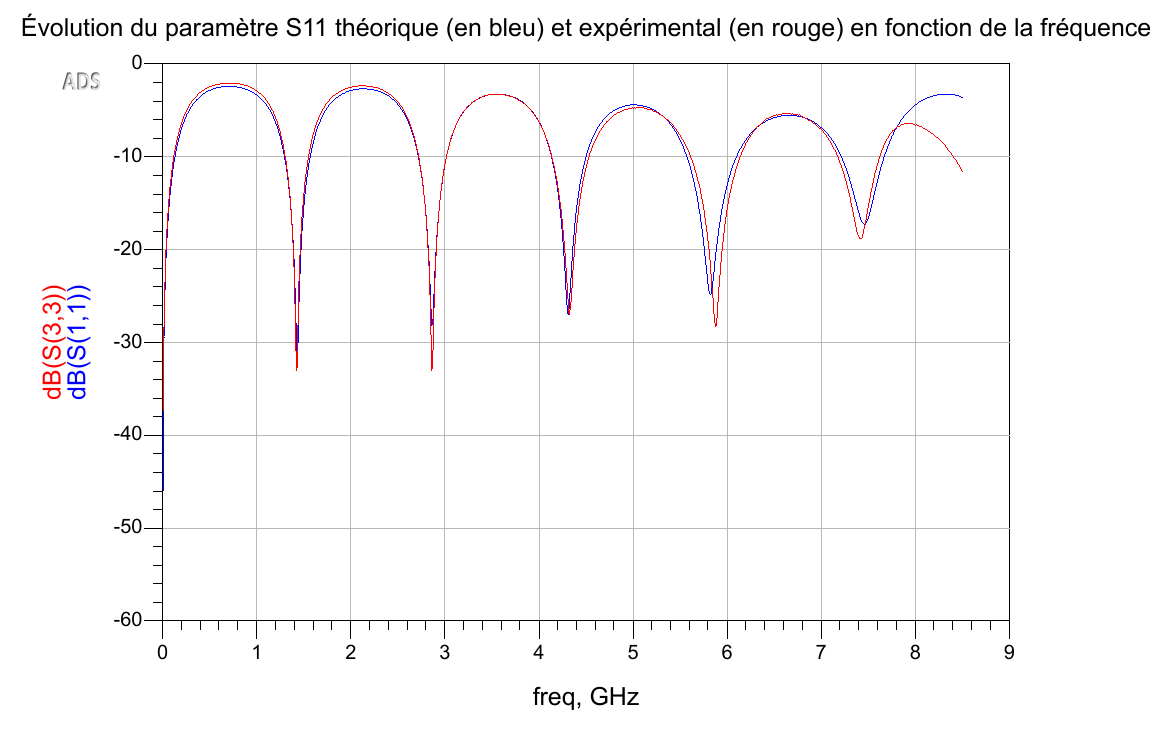
\includegraphics[scale=0.26]{../2carac/caract_large_bande/caract_teflonfin_t_17_micron.png}
	\caption{Graphique représentant les résultats de caractérisation large bande pour le téflon fin avec une hauteur de métallisation de 17 $\mu m$}
	\label{fig:amelioration_teflon_fin}
\end{figure}

Pour finir avec la caractérisation de ces lignes, il est possible de\\

Le logiciel fournit également un paramètre appelé la permittivité diélectrique relative effective $\varepsilon_{reff}$, déjà évoqué dans le rapport. Il s'agit d'une grandeur utile pour considérer le mode de propagation comme un mode quasi-TEM.

\begin{figure}[H]
	\centering
	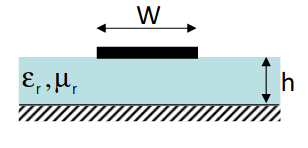
\includegraphics[scale=0.4]{../2carac/caract_large_bande/image_1_non_homogene.png}
	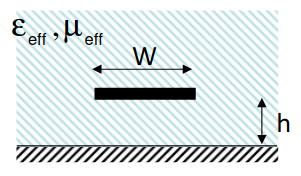
\includegraphics[scale=0.4]{../2carac/caract_large_bande/image_2_homogene.png}
	\caption{Schéma du principe d'homogénéisation de la constante diélectrique}
	\label{fig:homogeneisation_epsilon_reff}
\end{figure}

\newpage

\section{Synthèse de filtre passe-bas en technologie }


L'objectif est de réaliser un filtre passe-bas dont le gabarit est donné à la figure \ref{fig:gabarit_PasseBas} avec une réponse de Tchebychev.

\begin{figure}[H]
	\centering
	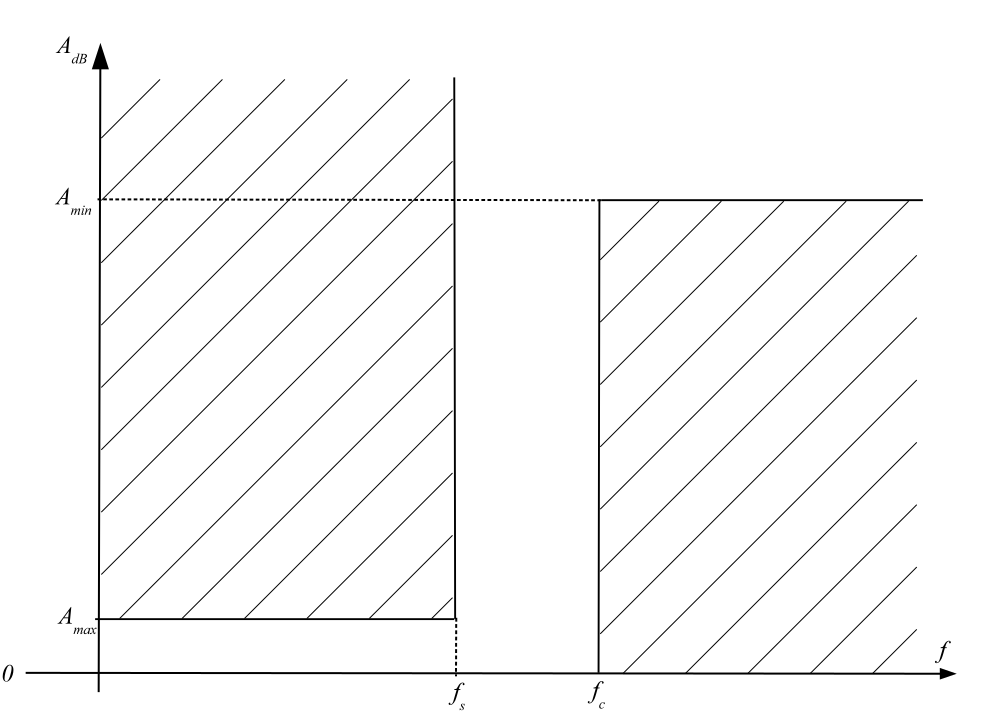
\includegraphics[width=0.5\linewidth]{ressources/gabarit_passe_bas}
	\caption{Gabarit filtre passe bas équivalent}
	\label{fig:gabarit_PasseBas}
\end{figure}

Les valeurs numériques associées au gabarit sont les suivantes.
\begin{table}[H]
	\centering
	\begin{tabular}{|c|c|c|c|}
		\hline
		$A_{max}$& $A_{min}$ & $f_s$ & $f_c$ \\ \hline
		0.1	dB & 15,00 dB 		& 2 GHz	   & 3 GHz \\ \hline
	\end{tabular}
	\caption{Valeur numérique gabarit souhaité}
\end{table}
La conception d'un filtre hautes fréquences débute par une synthèse classique avec des éléments passifs (condensateurs et bobines) comme il a été fait dans le module moyennes fréquences du S7. A partir du gabarit de la figure \ref{fig:gabarit_PasseBas}, l'équation ci-dessous nous est permet d'obtenir l'ordre du filtre à concevoir.


\begin{equation}
	n \geq \cfrac{argch(\sqrt{\cfrac{\alpha_{min}-1}{\alpha_{max} -1}})}{argch(1/k)}
\end{equation}
On rappelle :
\begin{equation}
argch(x)=ln(x+\sqrt{x^2-1})
\end{equation}

Où :
\begin{itemize}
	\item n est l'ordre du filtre souhaité;
		\item k est la sélectivité égal à : 
	\begin{equation}
	k=\frac{f_s}{1,5f_s} = \frac{2}{3} \approx 0,67
	\end{equation}
	\item $\alpha_{min}$ est l'atténuation minimale (en linéaire) du signal dans la bande atténué égal à $10^{\frac{15}{10}} \approx 31,6$
	\item $\alpha_{max}$ est l'atténuation maximale (en linéaire) du signal dans la bande passante égal à $10^{\frac{0,1}{10}} \approx 1,02$
\end{itemize}

L'application nous donne $n \geq 4,5$ soit au minimum un ordre 5 pour respecter le gabarit souhaité. Le schéma passe-bas en impédance que nous allons utiliser est donné ci-dessous par la figure \ref{fig:gabarit_PB}.

\begin{figure}[H]
	\centering
	\begin{circuitikz}
		\draw (0,0)
		to[V,v=$U_e$] (0,2) % The voltage source
		to[L=$g_1$] (2,2)
		to[C=$g_2$] (2,0) % The resistor
		(2,2)to[L=$g_3$] (4,2)
		to[C=$g_2$] (4,0) % The resistor
		(4,2)to[L=$g_3$] (6,2)
		to [R=$r$] (6,0) 
		to[short] (0,0);
	\end{circuitikz}
	\caption{Schéma prototype d'un filtre passe-bas de Tchebycheff en impédance.}
\end{figure}

Avec :
\begin{itemize}
	
	\item les coefficients $g_k$, les valeurs normalisées des condensateurs et des bobines;
	\item r, la résistance de charge normalisée est égale à 1. Sa valeur dénormalisé est de $50\Omega$;
	\item $U_e$, le signal d'entrée ayant une résistance série normalisée égale à 1 et donc $50\Omega$ en dénormalisée.
\end{itemize}

Pour obtenir les valeurs de $g_k$ nous ne pouvons utilisé les tableaux données dans le polycopié d'électronique moyennes fréquences car ils ne sont valables uniquement pour des ondulations de 0.5 dB et 1 dB. Notre gabarit nous impose une ondulation maximale de 0.1 dB dans la bande passante. Pour obtenir des coefficient $g_k$ qui permettent de respecter l'ondulation voulue nous avons réalisé un script sur Octave disponible en annexe. Le résultat obtenu est le suivant.

\begin{table}[H]
	\centering
	\begin{tabular}{|c|c|c|c|c|}
		\hline
		$g_1$ & $g_2$ & $g_3$ & $g_4$ & $g_5$\\
		\hline
		1.1468 & 1.3712 & 1.9750 & 1.3712 & 1.1468\\
		\hline
	\end{tabular}
	\caption{Valeurs des composants normalisées pour une ondulation de 0.1 dB}
	\label{tab:coefficient_g_k_passe_bas}
\end{table}
 
Pour trouver les valeurs réelles des composants il faut : pour les condensateurs, multiplier les $g_k$ pairs par un coefficient $C_{denom}$ et pour les bobines, multiplier les $g_k$ impairs par un coefficient $L_{denom}$. Les valeurs de ces coefficients sont données ci-dessous.

\begin{equation}
	C_{denom} = \frac{1}{2\pi f_s R}
	\qquad
	L_{denom} = \frac{R}{2\pi f_s}
\end{equation}

Le tableau ci-dessous donne les applications numériques pour les composants du filtre avec $f_c = 2GHz$ et $R = 50\Omega$.

\begin{table}[H]
	\centering
	\begin{tabular}{|c|c|c|c|c|}
		\hline
		$L_1$ & $C_2$ & $L_3$ & $C_4$ & $L_5$\\
		\hline
		4.56 nH & 2.18 pF & 7.86 nH & 2.18 pF & 4.56 nH\\
		\hline
	\end{tabular}
	\caption{Valeurs réelles des composants du filtre passe-bas.}
	\label{tab:valeurs_composant_passe_bas}
\end{table}


\begin{figure}[H]
	\centering
	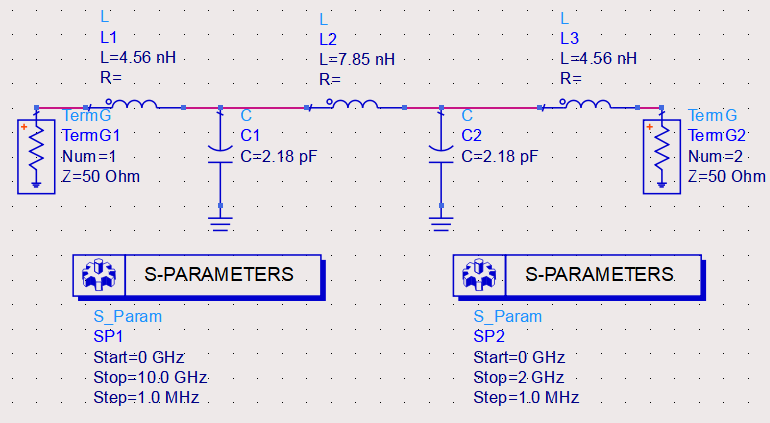
\includegraphics[width=9cm]{photo/passe_bas_vic/schema_localise_passe_bas_ads.png}
	\caption{Filtre passe-bas avec des éléments idéaux.}
	\label{fig:schema_localise_passe_bas_ads}
\end{figure}


\begin{figure}[H]
	\centering
	\begin{subfigure}[b]{0.49\textwidth}
		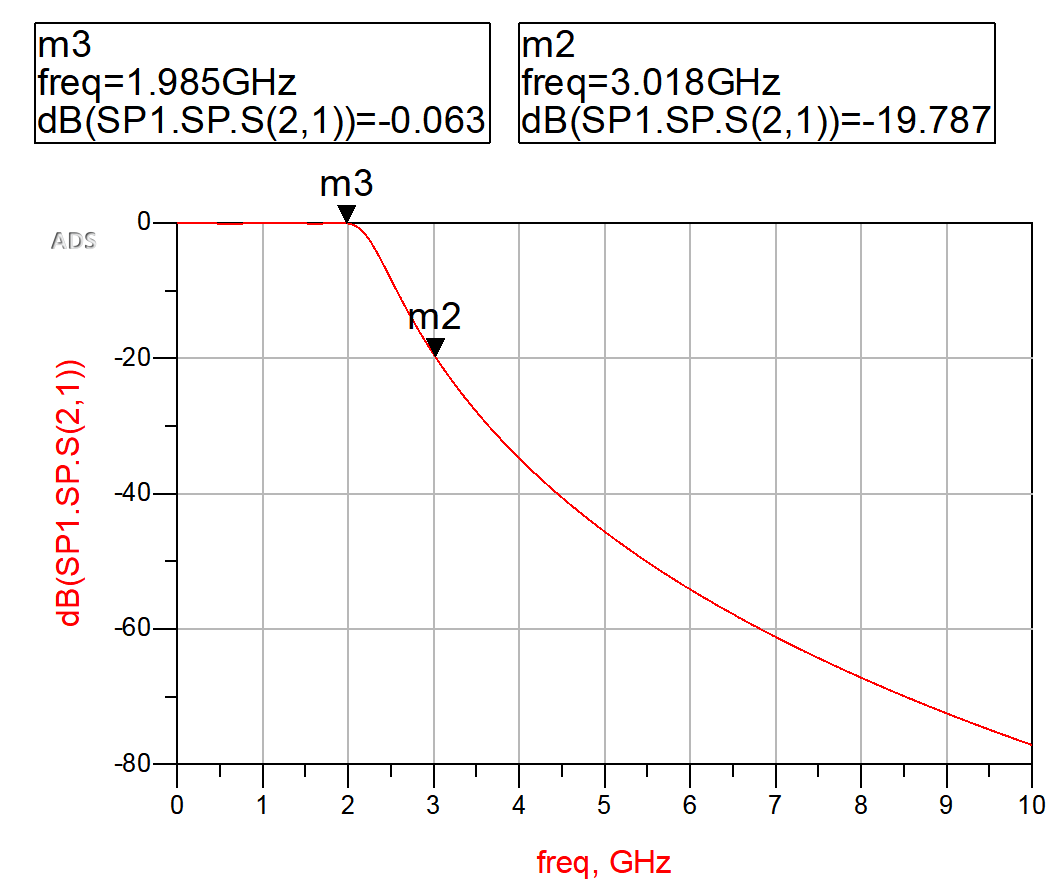
\includegraphics[width=\textwidth]{photo/passe_bas_vic/simu_passe_bas_localise.PNG}
		\caption{Sans zoom}
		\label{fig:simu_passe_bas_localise}
	\end{subfigure}
	\begin{subfigure}[b]{0.49\textwidth}
		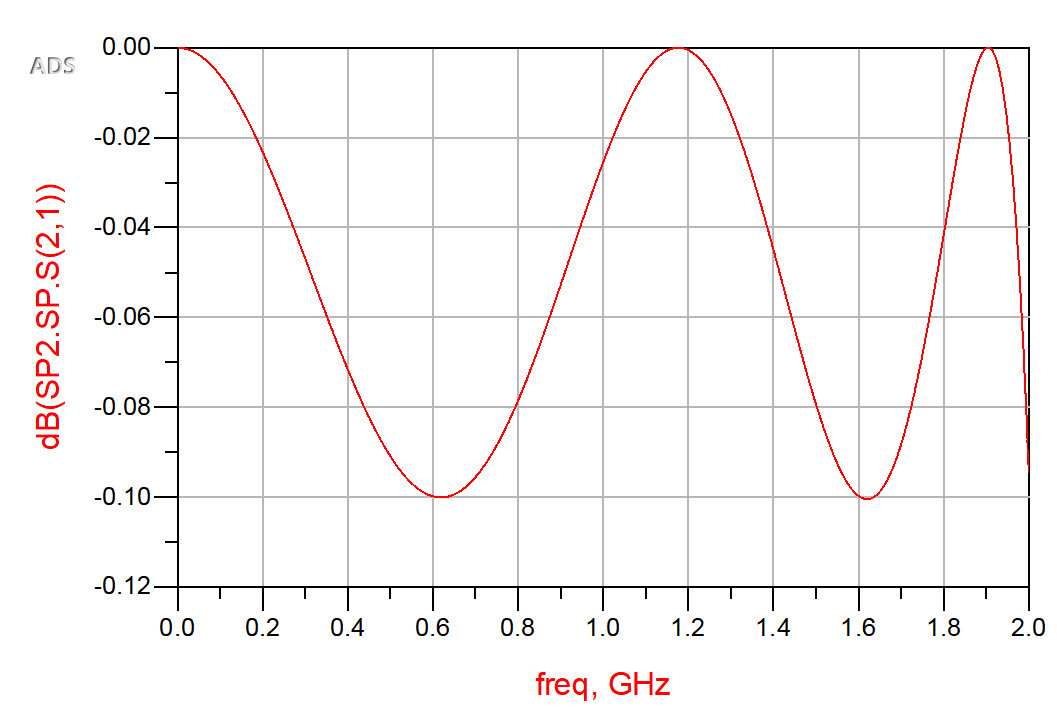
\includegraphics[width=\textwidth]{photo/passe_bas_vic/simu_zoom_passe_bas_localise.PNG}
		\caption{Avec zoom sur la bande passante}
		\label{fig:simu_zoom_passe_bas_localise}
	\end{subfigure}
	\caption{Simulation du module du coefficient de transmission S21 en dB}
%	\label{fig:observation_registres_internes}
\end{figure}


\begin{figure}[H]
	\centering
	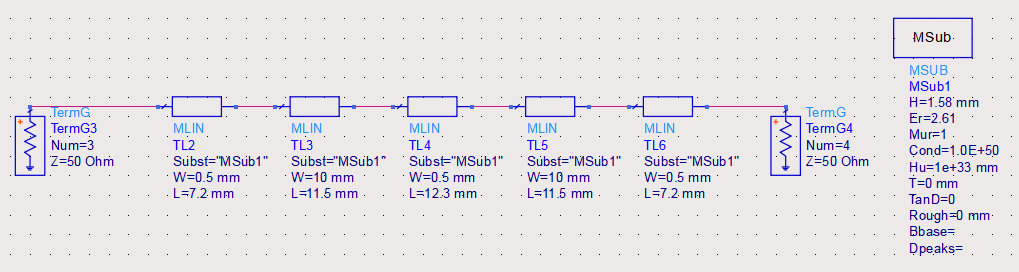
\includegraphics[width=15cm]{photo/passe_bas_vic/schema_distribue_passe_bas_ads.png}
	\caption{Filtre passe-bas en technologie micro ruban.}
	\label{fig:schema_distribue_passe_bas_ads}
\end{figure}



\begin{figure}[H]
	\centering
	\begin{subfigure}[b]{0.49\textwidth}
		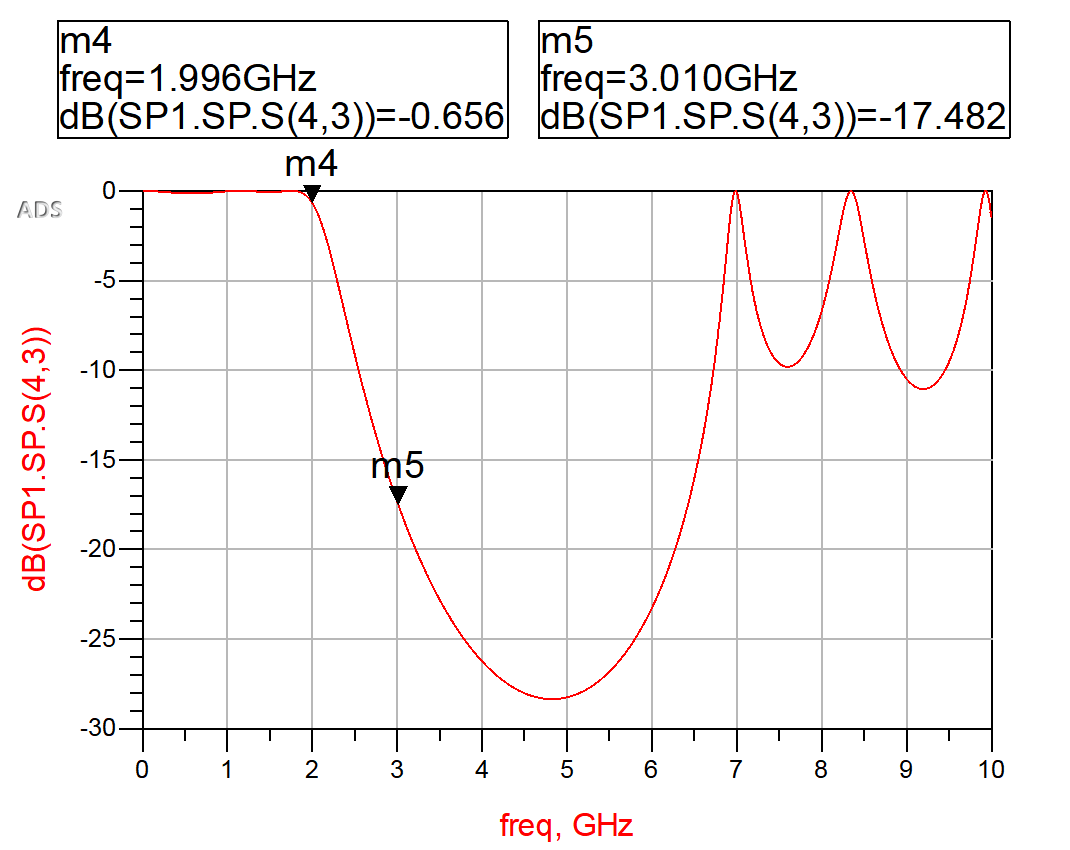
\includegraphics[width=\textwidth]{photo/passe_bas_vic/simu_passe_bas_distribue.PNG}
		\caption{Sans zoom}
		\label{fig:simu_passe_bas_distribue}
	\end{subfigure}
	\begin{subfigure}[b]{0.49\textwidth}
		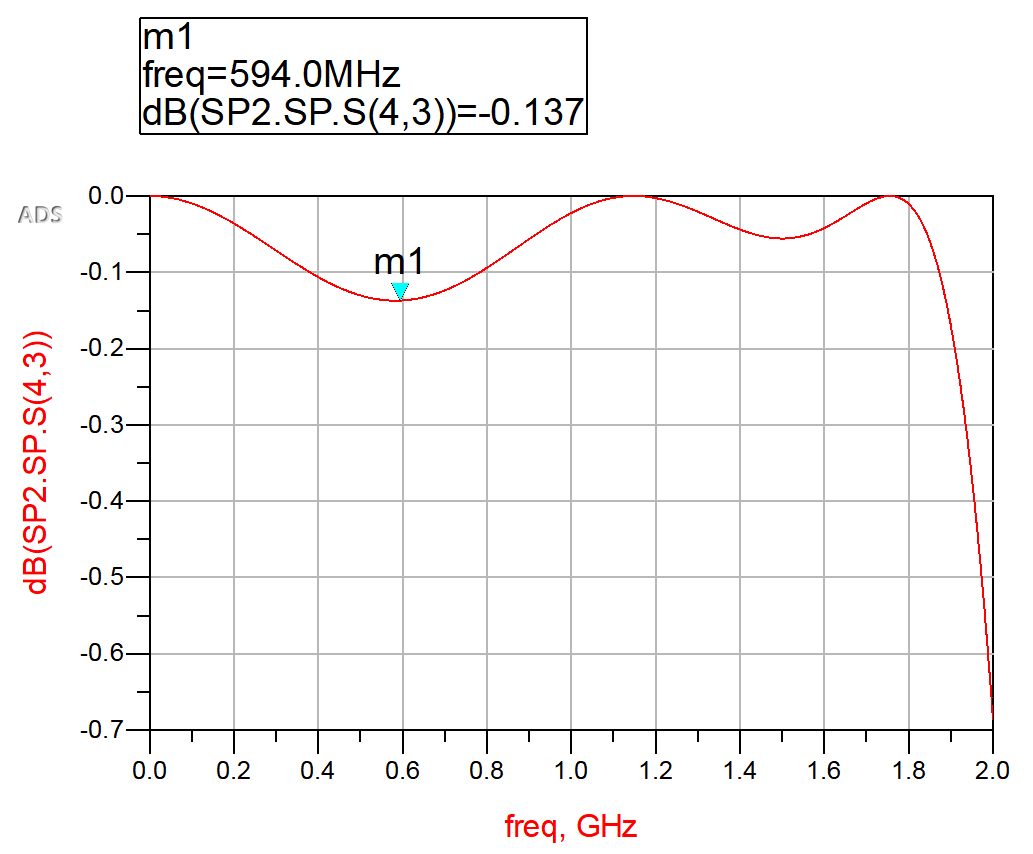
\includegraphics[width=\textwidth]{photo/passe_bas_vic/simu_zoom_passe_bas_distribue.PNG}
		\caption{Avec zoom sur la bande passante}
		\label{fig:simu_zoom_passe_bas_distribue}
	\end{subfigure}
	\caption{Simulation du module du coefficient de transmission S43 en dB}
	%	\label{fig:observation_registres_internes}
\end{figure}


\begin{figure}[H]
	\centering
	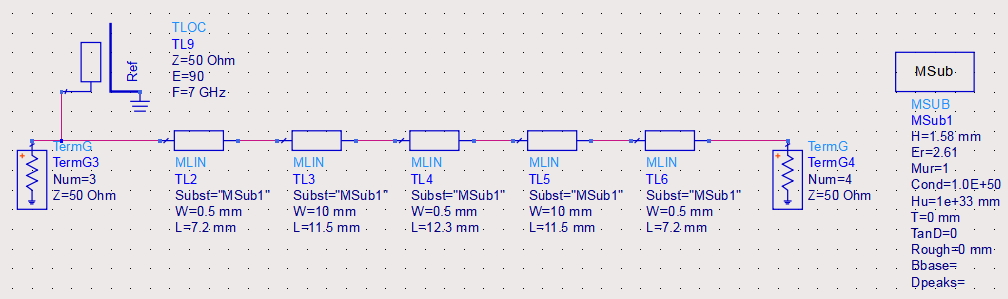
\includegraphics[width=15cm]{photo/passe_bas_vic/schema_distribue_ameliore_passe_bas_ads.png}
	\caption{Filtre passe-bas amélioré en technologie micro ruban.}
	\label{fig:schema_distribue_ameliore_passe_bas_ads}
\end{figure}


\begin{figure}[H]
	\centering
	\begin{subfigure}[b]{0.49\textwidth}
		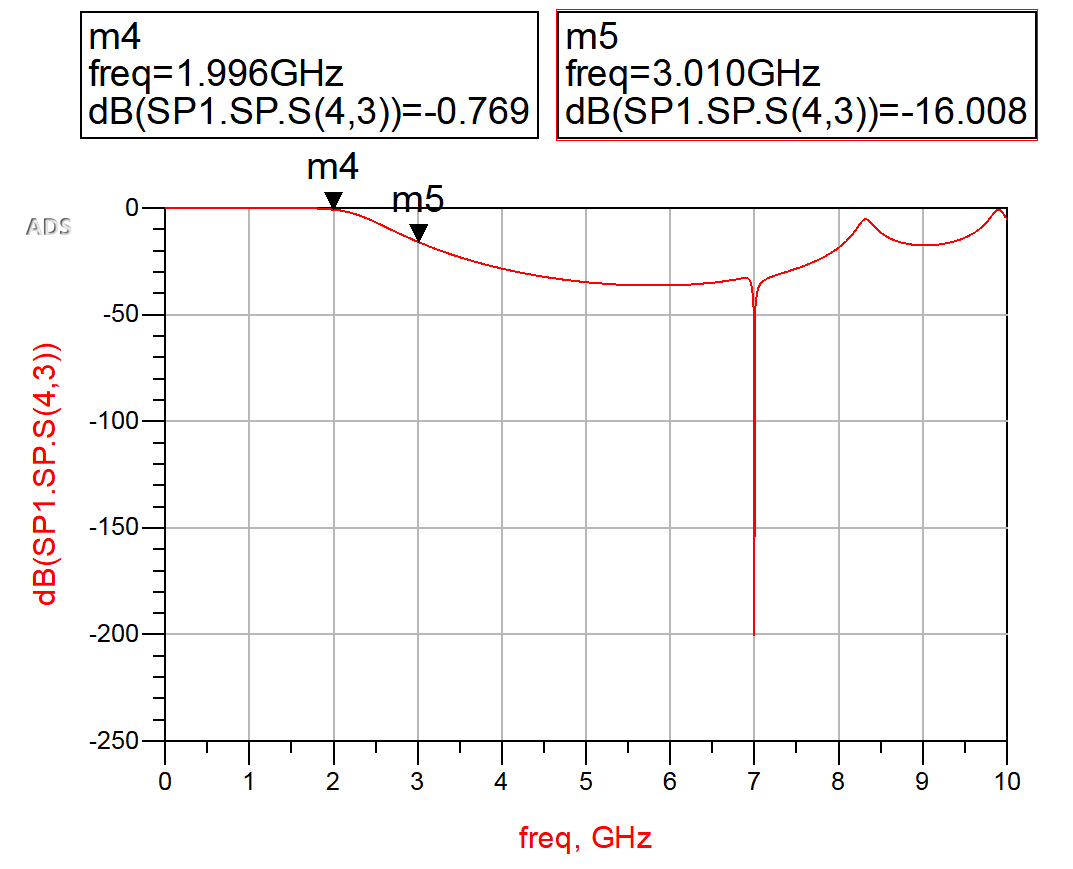
\includegraphics[width=\textwidth]{photo/passe_bas_vic/simu_passe_bas_distribue_ameliore.PNG}
		\caption{Sans zoom}
		\label{fig:simu_passe_bas_distribue_ameliore}
	\end{subfigure}
	\begin{subfigure}[b]{0.49\textwidth}
		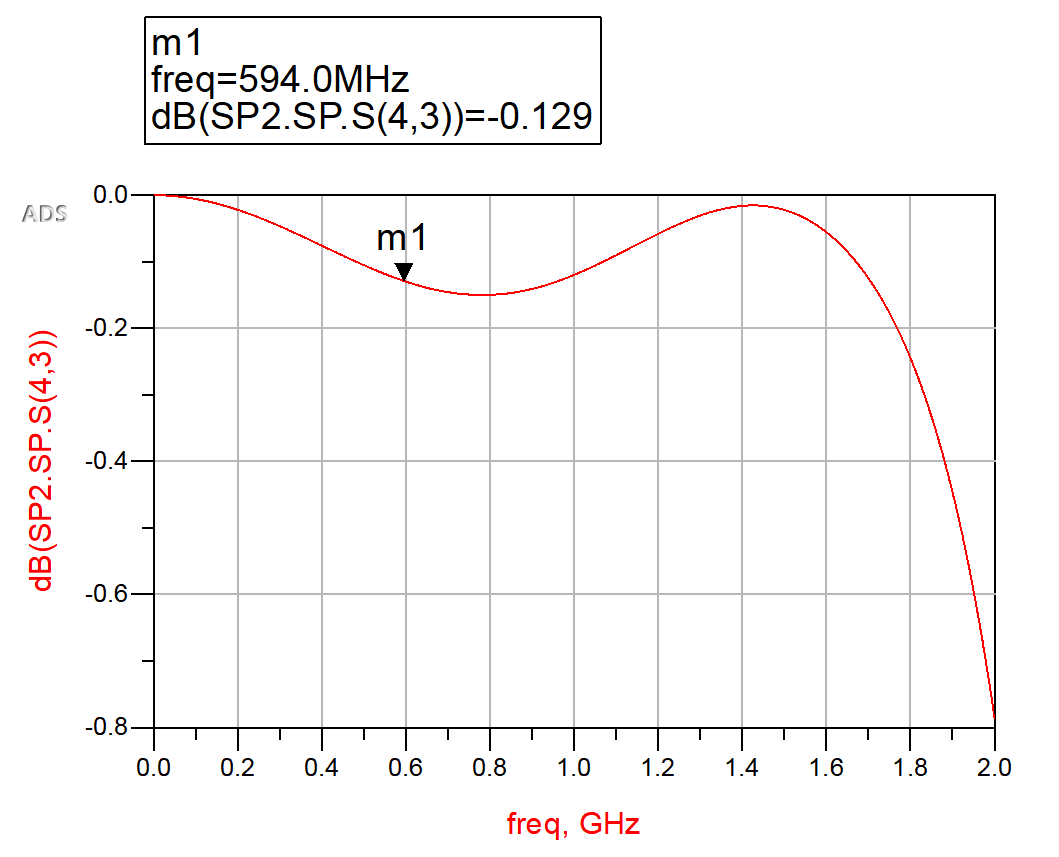
\includegraphics[width=\textwidth]{photo/passe_bas_vic/simu_zoom_passe_bas_distribue_ameliore.PNG}
		\caption{Avec zoom sur la bande passante}
		\label{fig:simu_zoom_passe_bas_distribue_ameliore}
	\end{subfigure}
	\caption{Simulation du module du coefficient de transmission S43 en dB}
	%	\label{fig:observation_registres_internes}
\end{figure}





\begin{figure}[H]
	\centering
	\begin{subfigure}[b]{0.49\textwidth}
		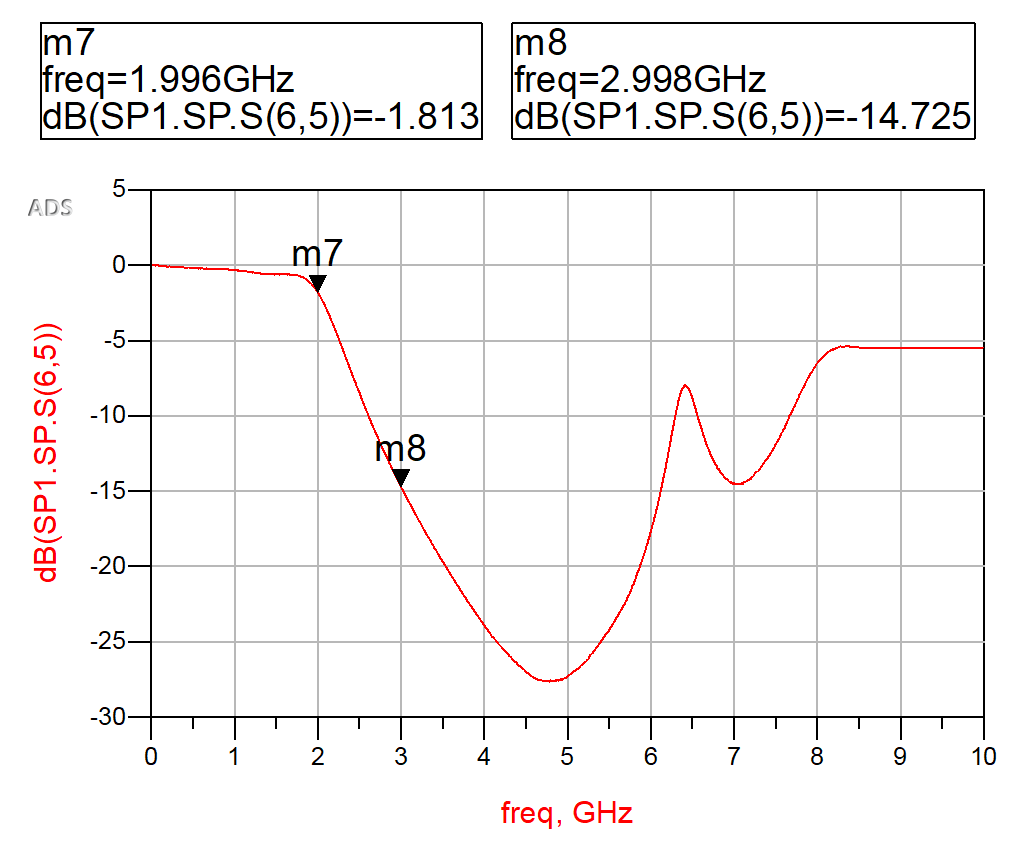
\includegraphics[width=\textwidth]{photo/passe_bas_vic/simu_passe_bas_reel_tche_epoxy.PNG}
		\caption{Sans zoom}
		\label{fig:simu_passe_bas_reel_tche_epoxy}
	\end{subfigure}
	\begin{subfigure}[b]{0.49\textwidth}
		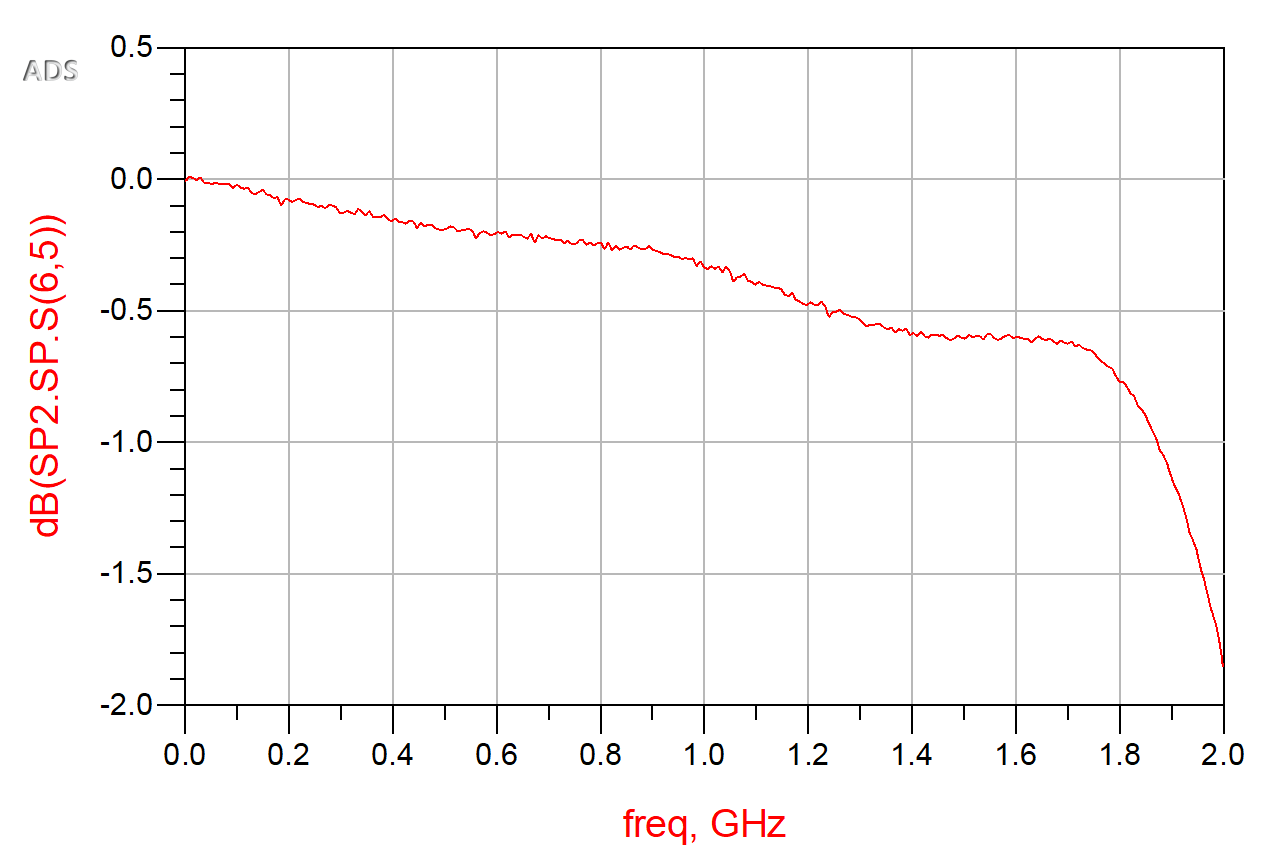
\includegraphics[width=\textwidth]{photo/passe_bas_vic/simu_zoom_passe_bas_reel_tche_epoxy.PNG}
		\caption{Avec zoom sur la bande passante}
		\label{fig:simu_zoom_passe_bas_distribue_ameliore}
	\end{subfigure}
	\caption{Module du coefficient de transmission S65 en dB d'un filtre passe-bas sur substrat epoxy}
	%	\label{fig:observation_registres_internes}
\end{figure}



\begin{figure}[H]
	\centering
	\begin{subfigure}[b]{0.49\textwidth}
		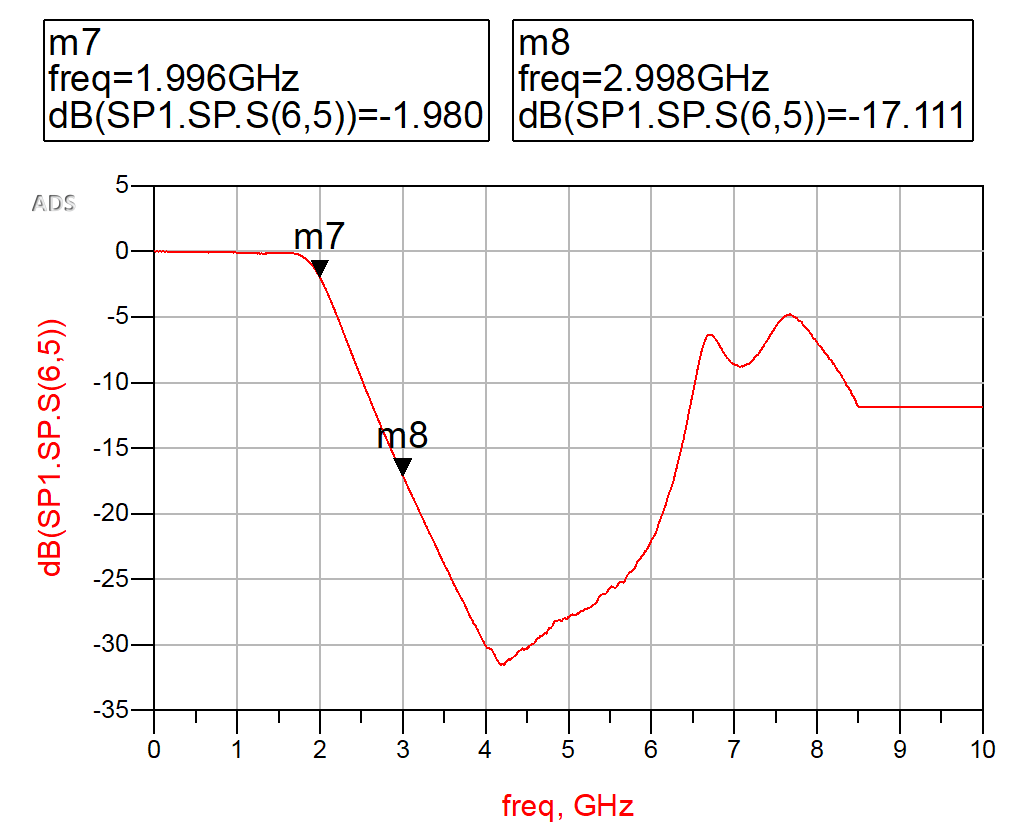
\includegraphics[width=\textwidth]{photo/passe_bas_vic/simu_passe_bas_reel_tche_teflon.PNG}
		\caption{Sans zoom}
		\label{fig:simu_passe_bas_reel_tche_teflon}
	\end{subfigure}
	\begin{subfigure}[b]{0.49\textwidth}
		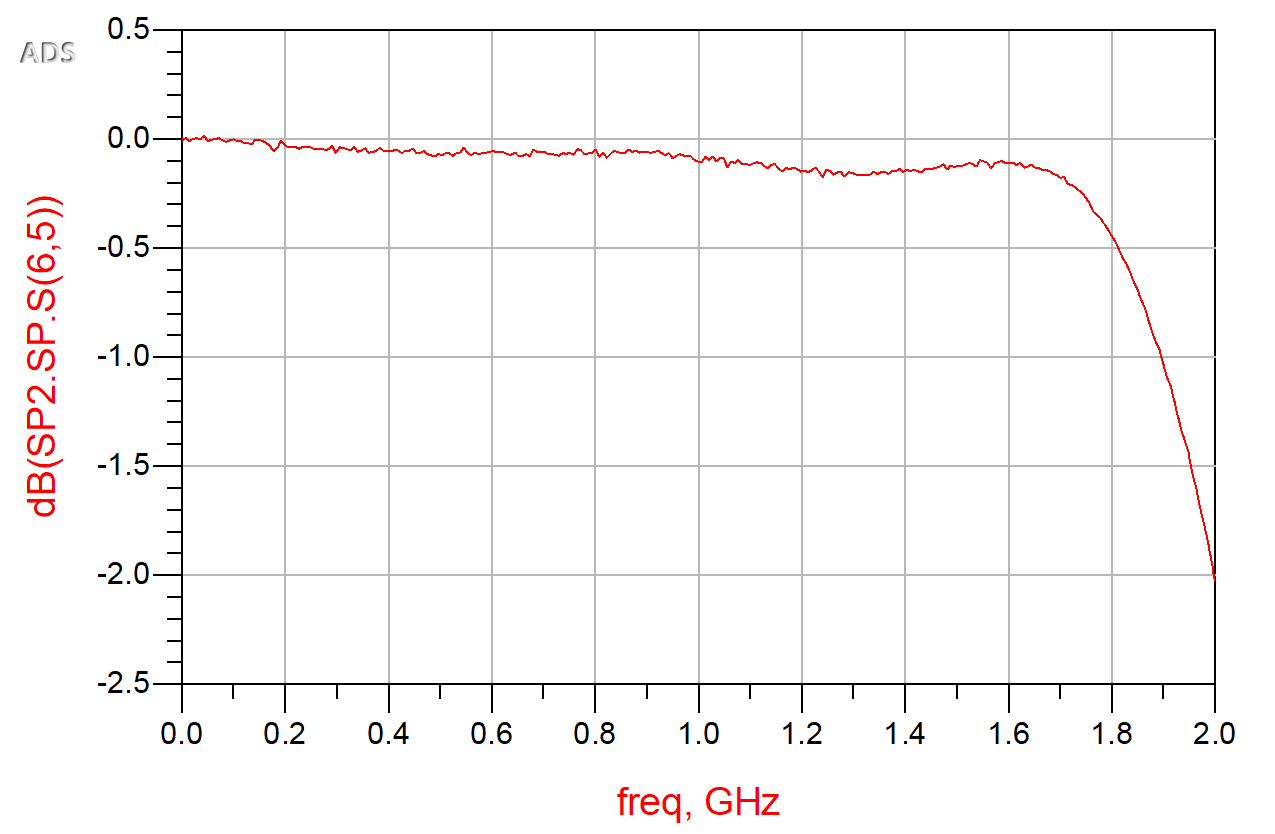
\includegraphics[width=\textwidth]{photo/passe_bas_vic/simu_zoom_passe_bas_reel_tche_teflon.PNG}
		\caption{Avec zoom sur la bande passante}
		\label{fig:simu_zoom_passe_bas_reel_tche_teflon}
	\end{subfigure}
	\caption{Module du coefficient de transmission S65 en dB d'un filtre passe-bas sur substrat teflon}
	%	\label{fig:observation_registres_internes}
\end{figure}




\section{synthèse d'un filtre passe-bande}

La synthèse d'un filtre en hautes fréquences à partir d'un gabarit se rapporte à la méthode étudiée en moyenne fréquence. Une étape finale est ajoutée permettant la transformation des éléments localisés en éléments distribués.
Le cahier des charges est le suivant, concevoir un filtre passe bande basé sur une fonction d'approximation de type Tchebychev et respectant le gabarit figure \ref{fig:gab}. L'implémentation réelle doit se en utilisant exclusivement des lignes micro ruban de longueur $\lambda_g/2$ ou $\lambda_g/4$ et des stubs.

\begin{figure}[H]
	\centering
	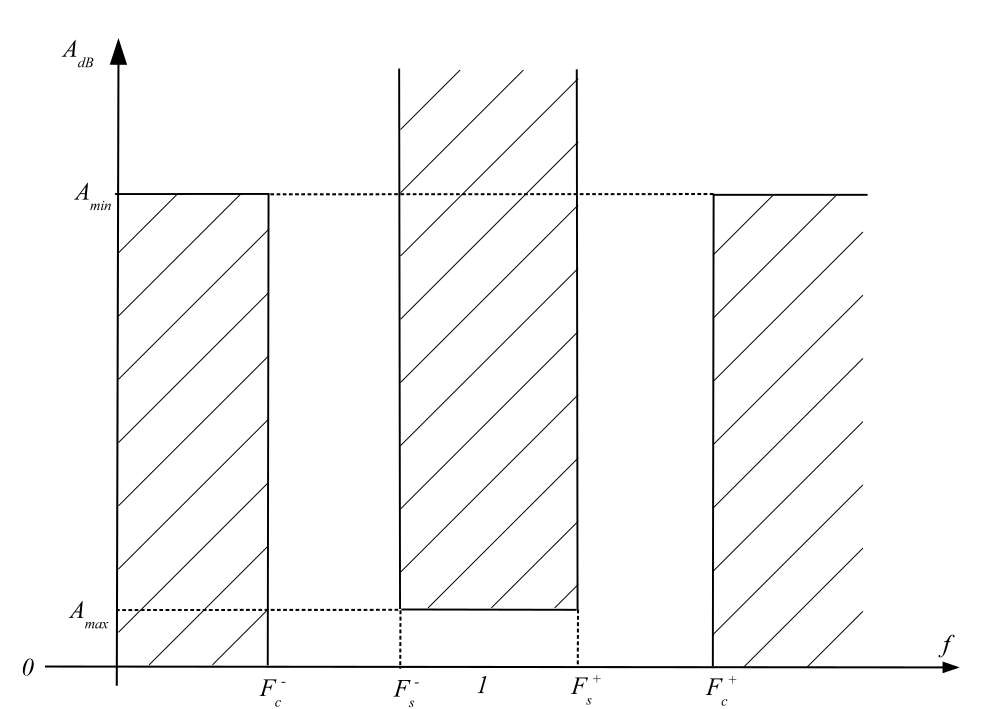
\includegraphics[width=0.5\linewidth]{ressources/gabarit_passe_bande}
	\caption{Gabarit du filtre passe-bas souhaité}
	\label{fig:gab}
\end{figure}
Les valeurs numériques associées au gabarit sont les suivantes. Les fréquences sont en GHz et l'atténuation en dB. 
	\begin{table}[H]
		\centering
\begin{tabular}{|c|c|c|c|c|c|}
		\hline
	$A_{max}$& $A_{min}$ & $f_c^-$ & $f_s^-$ & $f_s^+$ &$f_c^+$ \\ \hline
	0,1000	 & 15,00 		& 1,500	   & 1,750 & 2,250& 3,000 \\ \hline
	\end{tabular}
\caption{Valeur numérique gabarit souhaité}
	\end{table}
\paragraph{Symétrie du gabarit} ~~\\ \noindent
Avant de commencer la synthèse du filtre il est nécessaire de valider une condition sur la symétrie. Si elle n'est pas respectée il faudra modifier le gabarit du cahier des charges. La condition s'opère sur la moyenne géométrique de la bande passante et de la bande coupée notées :
\begin{equation}
	 f_{co} = \sqrt{f_c^-.f_c^+}, \quad f_{so} = \sqrt{f_s^- f_s^+}
\end{equation}
Ainsi, si $f_{so} = f_{co}$, le gabarit est centré il n'est pas nécessaire de réaliser d'opération particulaire. On obtient a alors  $f_{so} = f_{co} = f_0$ avec $f_0$ la fréquence centrale du gabarit. Si $f_{so} \neq f_{co}$, le gabarit n'est pas centré il faut passer par une étape de centrage du gabarit avant de réaliser la synthèse du filtre.\\
Application numérique :\\
\begin{equation}
f_{co} = \sqrt{f_c^-.f_c^+} = \sqrt{1,500*3,000} = 2,121 GHz
\end{equation}
\begin{equation}
	f_{so} = \sqrt{f_s^- f_s^+} = \sqrt{1,750*2,250} = 1,984 GHz
\end{equation}
\begin{equation}
f_{so} <	f_{co}
\end{equation}
Le filtre est asymétrique il faut réaliser l'opération de centrage. Dans notre cas elle vise à diminuer $f_{co}$. Il est possible de faire varier la borne positive $f_c^+$. Cela à pour effet de sur contraindre le cahier des charges. Pour répondre aux exigences il est interdit d'élargir la bande atténué ou de diminuer la bande passante. Ainsi on fixe la fréquence centrale $f_0 = f_{so} = \sqrt{f_s^- f_s^+}$.  
Il vient donc :
\begin{equation}
f_c^+=\frac{f_{so}^2}{f_c^-}=\frac{1,984^2}{1,500}=2,614GHz
\end{equation}
Les nouvelles valeurs numériques pour le gabarit du filtre sont les suivantes. Elle font référence à la figure \ref{fig:gab}.
	\begin{table}[H]
	\centering
	\begin{tabular}{|c|c|c|c|c|c|c|}
		\hline
		$A_{max}$& $A_{min}$ & $f_c^-$ & $f_s^-$ & $f_0$ & $f_s^+$ &$f_c^+$ \\ \hline
		0,1000		 & 15,00 		& 1,500	   & 1,750 & 1,984 & 2,250& 2,614 \\ \hline
	\end{tabular}
	\caption{Valeur numérique gabarit centré}
\end{table}
\paragraph{Gabarit passe bas} ~~\\ \noindent
L'étape suivant dans la conception d'un filtre passe bande symétrique vise à simplifier la synthèse en passant par un gabarit passe bas. Cela permet de calculer son ordre puis sa structure en éléments localisés.
\begin{figure}[H]
	\centering
	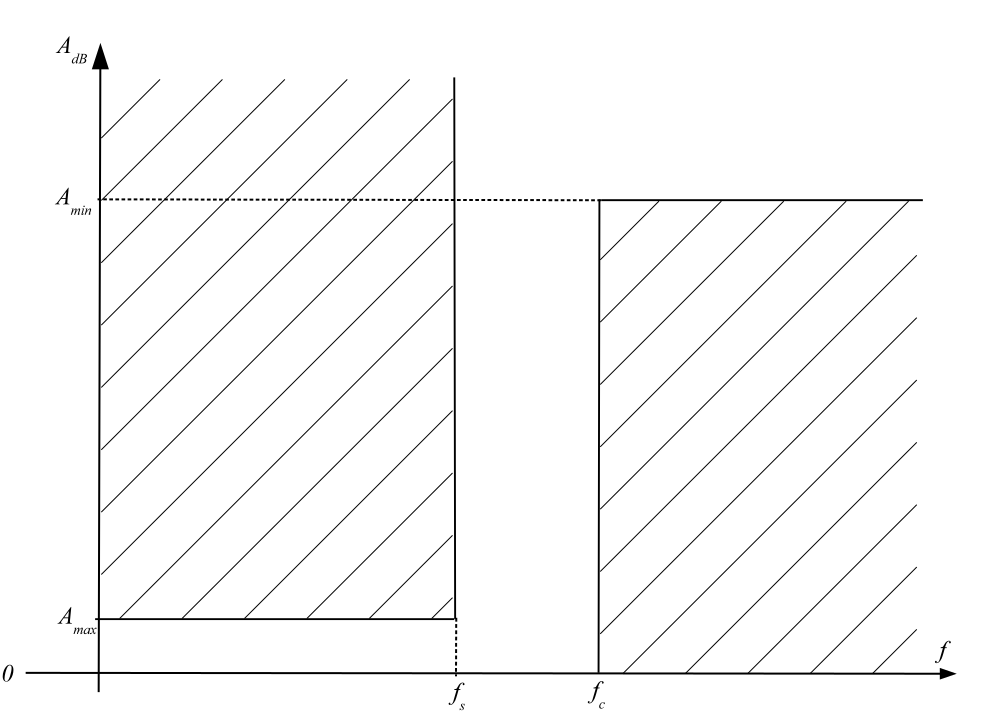
\includegraphics[width=0.5\linewidth]{ressources/gabarit_passe_bas}
	\caption{Gabarit filtre passe bas équivalent}
	\label{fig:gabaritpassepas}
\end{figure}
L'évaluation du coefficient de sélectivité permet d'établir le gabarit normalisée. Cette grandeur se note $k$ est sans unité et strictement inférieure à 1. Son expression est la suivante :
\begin{equation}
	k=\frac{\Delta.f_s}{\Delta.f_c}=\frac{f_s^+-f_s^-}{f_c^+-f_c^-}=\frac{2,250-1,75}{2,614-1,500}=0,4488
\end{equation}
L'ordre du filtre $\delta \in N$ est donnée pour une fonction d'approximation de Tchebychev avec l'expression suivante. Les atténuations $A_{min}$ et $A_{max}$ en dB correspondent respectivement aux fréquences $f_s$ et $f_c$.
\begin{equation}
\delta \geq \frac{argch
	\Big( \sqrt{\cfrac{10^{A_{min}/10}-1}{10^{A_{max}/10}-1}}
	\Big)
}{argch(1/k)}
\end{equation}
On rappelle pour la calculatrice :
\begin{equation}
argch(x)=ln(x+\sqrt{x^2-1})
\end{equation}
On calcule avec $A_{min} = 15dB$ et $A_{max} = 0,1dB$. L'ordre $\delta$ est arrondi à l'entier supérieur.
\begin{equation}
\frac{argch
	\Big( \sqrt{\cfrac{10^{15/10}-1}{10^{0,1/10}-1}}
	\Big)
}{argch(1/0,4488)} = 2,975, \quad \delta = 3
\end{equation}
Le gabarit impose un ordre minimum de 3, c'est la valeur que nous retiendront. On note tout de même que l'arrondi au supérieur présente un faible écart avec l'ordre choisi. Notre filtre devrait respecter les spécifications mais des approximations pourraient entraîner des débordements notamment aux fréquences particulières $f_c$ et $f_s$.
\paragraph{Prototype passe bas normalisé vers passe bande dénormalisé} ~~\\ \noindent
Cette étape vise à transformer le schéma passe bas en son équivalent passe bande. Il existe deux schémas possibles dit de type impédance et de type admittance où, respectivement, le premier élément est une inductance ou un condensateur. Le cahier des charges ne donne pas d'indications sur ce point. Nous choisirons le schéma qui a l'avantage de simplifier la transposition micro ruban.
\begin{figure}[H]
	\centering
	\begin{circuitikz}[scale=0.8]
		\draw 
		(0,0) to[esource] (0,2) % The voltage source
		to [R=$1$] (3,2) 
		to[L=$l'_1$] (5,2)
		to[L=$l'_3$] (8,2)
		to [R=$r$] (8,0) 
		to[short] (0,0)
		(5.3,2)to[C=$c'_2$] (5.3,0);
	\end{circuitikz}
	\caption{Schéma prototype filtre passe-bas ordre 3 en impédance}
	\label{fig:ordre3_LP_adm}
\end{figure}
La figure \ref{fig:ordre3_LP_adm} représente le prototype du filtre passe bas. Il est composé de trois composants réactifs et le premier est une self, nous sommes bien en présence d'un filtre d'ordre trois de type impédance. Les valeurs normalisées de ces composants s'expriment à partir de l'atténuation maximum $A_{max}$, de l'ordre du filtre et de la charge. Dans le cas des ordres paires les deux résistances n'ont pas la même valeur, il est donc préférable de choisir un ordre impaire sans quoi une problématique d'adaptation se posera. Les calculs pour obtenir les valeurs des composants sont détaillés dans \cite{cours_MF} à la page 93. Ils font intervenir des fonctions trigonométriques relativement complexes. La figures \ref{fig:coefnormaliseondulation01db} ci-dessous rassemble ces grandeurs et nous évite les calcul. Elle correspond  à une ondulation inférieur à 0,1dB en bande passante et un ordre compris entre 1 et 10. 
\begin{figure}[H]
	\centering
	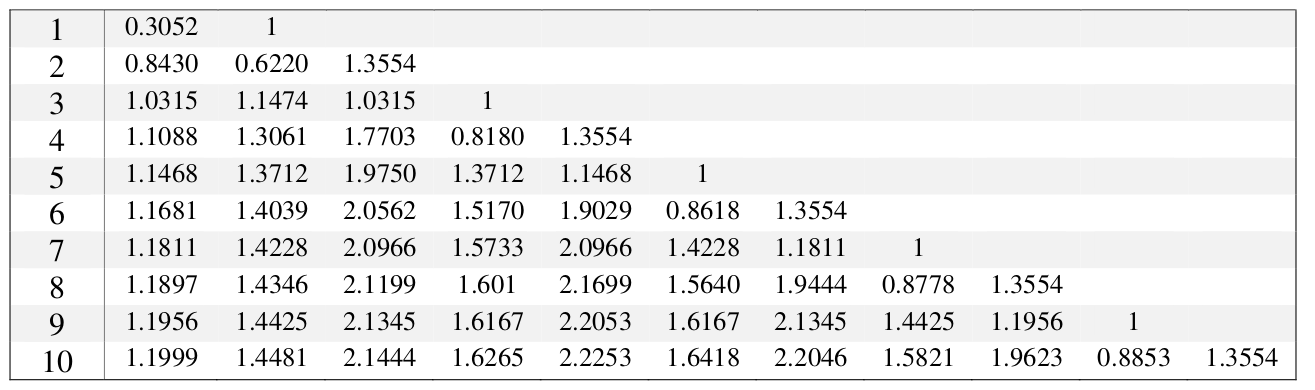
\includegraphics[width=0.8\linewidth]{ressources/coef_normalise_ondulation01dB}
	\caption{Coefficients normalisés fonction de Tchebychev 0,1dB ondulation}
	\label{fig:coefnormaliseondulation01db}
\end{figure}
La première colonne de ce tableau correspond à l'ordre du filtre. Les valeurs suivantes correspondent aux composants de gauche à droite sur le schéma. La dernière valeur concerne la résistance de charge. On remarque bien que pour les ordres impaire cette dernière vaut l'unité contrairement aux ordres impaires. Dans notre cas $l'_1=1,0315$, $c'_2=1,1474$ et $l'_3=1,0315$. Les informations nécessaires à la transformation du schéma équivalant passe bas au schéma équivalent passe bande ont été rassemblé. Nous pouvons opérer cette opération. Les éléments inductifs doivent être remplacés par une self et un condensateur en série. Les éléments capacitifs doivent être remplacés par une self et un condensateur en parallèle. Les valeurs normalisées des nouveaux composants sont données par les expressions suivantes:\\
Cas de l'inductance :
\begin{equation}
c_k=\frac{B}{l'_k}, \quad l_k=\frac{l'_k}{B}, \quad k = \{1,3\}
\end{equation}
Cas du condensateur :
\begin{equation}
c_k=\frac{c'_k}{B}, \quad  l_k=\frac{B}{c'_k}, \quad k = \{2\}
\end{equation}
Où B désigne la bande passante
\begin{equation}
	B=\frac{\Delta f_s}{f_0}=\frac{f_s^+-f_s^-}{f_0}=\frac{2,250-1,75}{1,984}=0,2520
\end{equation}
Le schéma du filtre passe bande en éléments localisés après transformation est illustré par la figure \ref{fig:ordre3_BP_imp}.

\begin{figure}[H]
	\centering
	 \ctikzset{bipoles/length=1.1cm}
	\begin{circuitikz}[scale=0.85]
		\draw 
		(0,0) to[esource] (0,3) % The voltage source
		to [R=$1$] (2,3) 
		to[L=$l_1$] (4,3)
		to[C=$c_1$] (6,3)
		to[L=$l_3$] (8,3)
		to[C=$c_3$] (10,3)
		to [R=$r$] (10,0) 
		to[short] (0,0)
		(6,3) to[short] (6,2.5)
		(5.5,2.5) to[short] (6.5,2.5)
		(5.5,2.5) to[L=$l_2$] (5.5,0.5)
		(6.5,2.5) to[C=$c_2$] (6.5,0.5)
		(5.5,0.5) -- (6.5,0.5)
		(6,0.5) -- (6,0);
	\end{circuitikz}
	\caption{Schéma filtre passe-bande ordre 3 en impédance}
	\label{fig:ordre3_BP_imp}
\end{figure}
A partir des expression précédente il est possible de calculer les valeurs normalisée de ces nouveaux composants. Nous pouvons pas le même occasion opérer la dénormalisation. Les grandeurs dénormalisées seront notées en majuscule. De nouveau on s'appuis sur le cours d'électrique moyenne fréquence \cite{cours_MF}. On y extrait les égalités suivantes :
\begin{equation}
C_k = \frac{c_k}{2\pi f_0.R},
\quad
L_k = \frac{l_k.R}{2\pi .f_0},
\quad
k=\{1,2,3\}
\end{equation}
On prendra la résistance de charge valant $50\Omega$ et la fréquence centrale $f_0$ 1,984GHz. Un petit programme Octave nous permet d'automatiser ce calcul. Les résultats de l'étape de transformation et de dénormalisation sont rassemblés dans le tableau \ref{tab:denorm_BP}. On rappel que la notation utilisée représente les grandeurs normalisées en minuscule et les grandeurs dénormalisées en majuscule.

\begin{table}[H]
	\centering
	\begin{tabular}{|c|c|c|c|}
		\hline
		k & 1 & 2 & 3 \\
		\hline
		$c_k$ & 0,2443 & 4,553 & 0,2443 \\ \hline
		$l_k$ &	4,093	&	0,2196	&	4,093	\\ \hline
		$C_k$ &	0,3917pF&	7,307pF	&	0,3917pF\\ \hline
		$L_k$ &	16,42nH	&	0,8804nH& 16,42nH	\\ \hline
	\end{tabular}
	\caption{Valeurs passe bande avant et après dénormalisation}
	\label{tab:denorm_BP}
\end{table}
%\begin{table}[H]
%	\centering
%	\begin{tabular}{|c|c|c|c|}
%		\hline
%		k & 1 & 2 & 3 \\
%		\hline
%		$c_k$ & 0,2443 & 4,553 & 0,2443 \\ \hline
%		$l_k$ &	4,093	&	0,2196	&	4,093	\\ \hline
%		$C_k$ &	0,3919pF&	7,303pF	&	0,3919pF\\ \hline
%		$L_k$ &	16,41nH	&	0,8808nH& 16,41nH	\\ \hline
%	\end{tabular}
%	\caption{Valeurs passe bande avant et après dénormalisation}
%	\label{tab:denorm_BP}
%\end{table}
Afin de valider les valeurs obtenue nous pouvons recourir à une simulation sur ADS. Le schémas tracé est illustré par la figure \ref{fig:ads_sch_BP_localise}.
\begin{figure}[H]
	\centering
	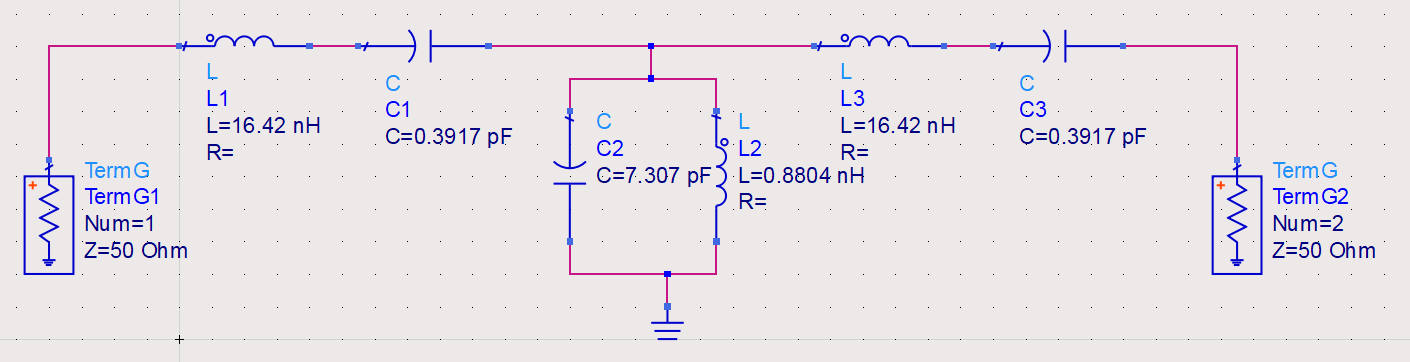
\includegraphics[width=0.9\linewidth]{../4synthPBande/impedance/schema_passe_bande_localise}
	\caption{Schéma passe bande ADS}
	\label{fig:ads_sch_BP_localise}
\end{figure}
Il fait intervenir des composants de la bibliothèque "lumbed component". La simulation porte sur l'observation des paramètres S et plus particulièrement du coefficient de transition $S_{21}$. Le résultat obtenue est donné par la deux figure \ref{fig:ads_S21_BP_localise1}. Elles permettent respectivement de vérifier la coupure et l'ondulation en bande passante.
\begin{figure}[H]
	\centering
	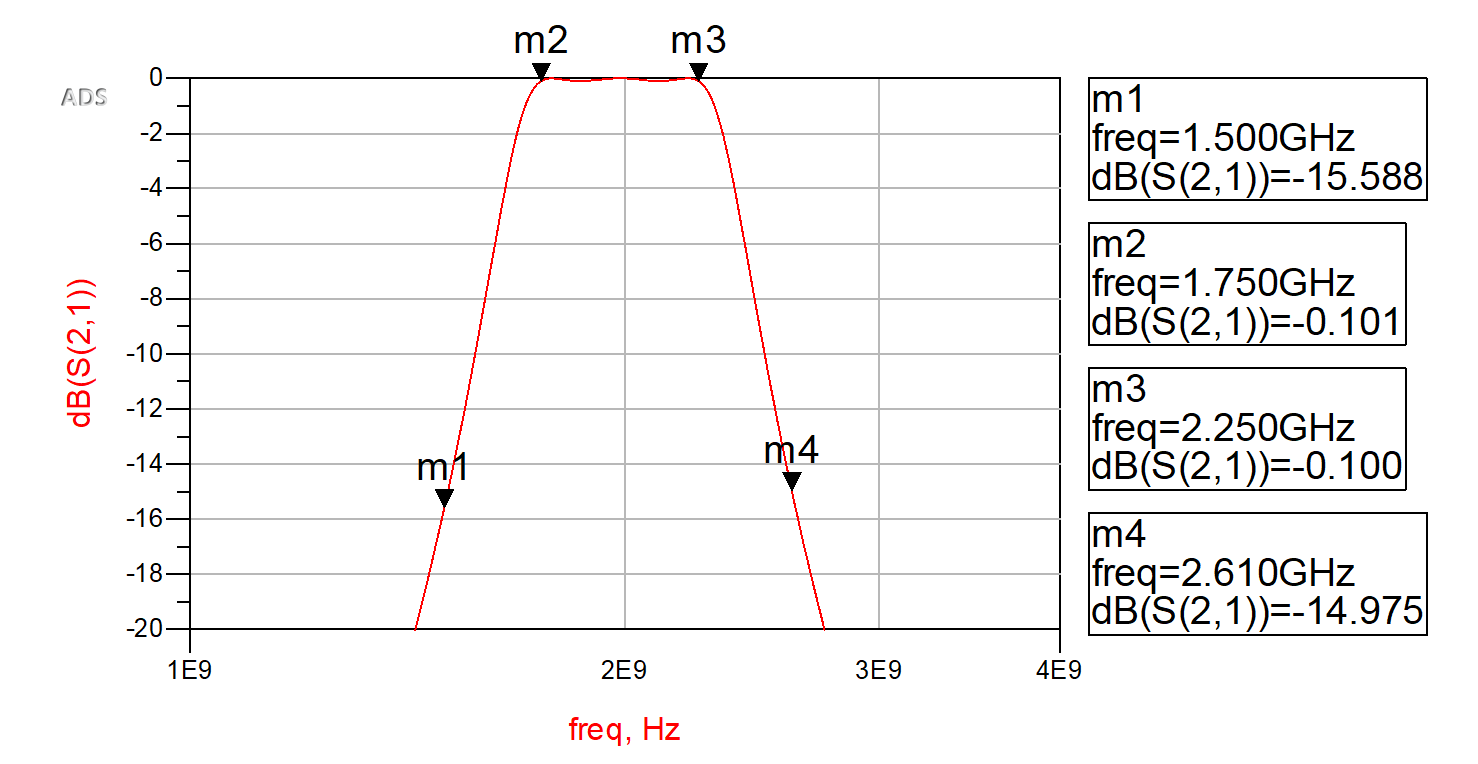
\includegraphics[width=0.49\linewidth]{../4synthPBande/impedance/S21__passe_bande_localise}
	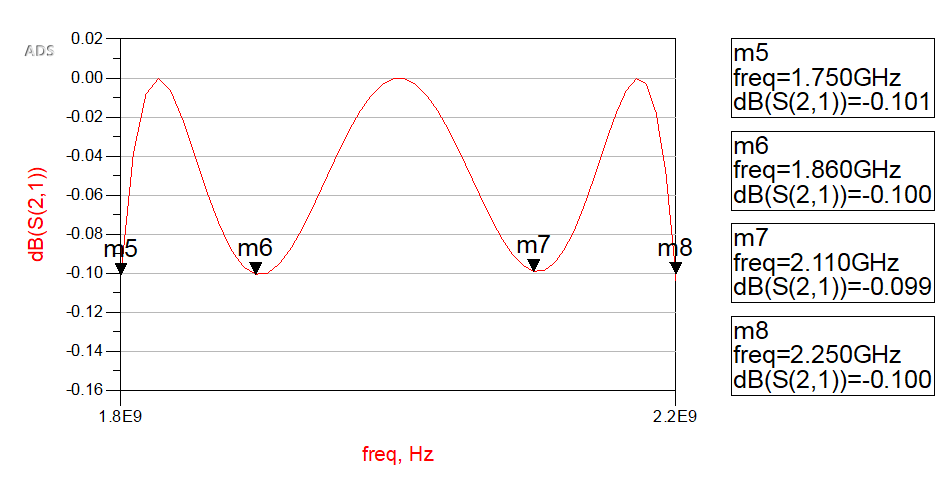
\includegraphics[width=0.49\linewidth]{../4synthPBande/impedance/S21__bande_passante_passe_bande_localise}
	\caption{Simulation S21 passe bande localisé}
	\label{fig:ads_S21_BP_localise1}
\end{figure}
La figure de gauche représente le paramètre S21 en db sur la bande spécifiée par le gabarit. On relève une atténuation de 15,58dB et 14,97dB au points m1 et m4. Seul le premier garantie respect strictement le cahier des charges. La figure de gauche représente elle aussi le coefficient de transition mais sur une bande plus étroite correspondant à la bande passante. La condition du gabarit spécifie une ondulation inférieur à 0,1dB. Elle est respecter partout sauf au point m5 où on relève 0,101dB. Les résultats de cette simulation présentes deux débordement débordements aux fréquences particulières $f_c^-$ et $f_s^-$. Cela s'explique par une approximation réalisée lors du centrage du gabarit. En effet, seule la borne $f_c^+$ a été déplacée se qui entraîne une légère dysmétrie entre le gabarit initial et celui recentré. Aussi, nous avons pu remarqué que l'ordre du filtre décimal est très proche de la valeur entière retenue ce qui a pour effet de laisser peu de marge aux fréquences particulières. Ces deux éléments cumulés ont joué en notre défaveur en aboutie à une synthèse en limite de spécification. 
Il existe une méthode détaillée dans le \textit{cours de filtrage actif} de Vincent Gouret faisant varier à la fois $f_c^+$ et $f_c-$ lors du recentrage. Cette méthode est plus complexe mais aurait probablement permise de réaliser une synthèse répondant parfaitement au gabarit.\\
Les résultats de simulation reste malgré tout concluant car ils présentent une erreur très faible. Nous conserverons donc les valeurs des composants pour la suite des calculs.\\

Les valeurs dénormalisées obtenues devrait permettre en théorie de constituer un filtre passe bande en éléments localisés. Cependant en pratique l'ordre de grandeur (0,1pF pour les condensateurs et 1nH pour les inductances) pose un problème de provisionnement. En effet, elles sont peu réaliste puisque comparables aux phénomènes parasites des boîtiers et conducteurs. Il est possible de résoudre ce problème en transformant cette synthèse localisé en synthèse distribuée.

\subsection{title}
Il existe plusieurs circuits basés sur les propriété des lignes pour réalisé un filtre passe bande. Nous détaillerons deux solutions basées uniquement sur des lignes $\lambda /2$ et $\lambda /4$. 

\section{Conclusion}
Il existe une méthode détaillée dans le \textit{cours de filtrage actif} de Vincent Gouret faisant varier à la fois $f_{so}$ et $f_{co}$. Elle permet d'optimiser la contrainte sur le sélectivité. 












Une fois le coefficient de dénormalisation appliqué nous obtenons les valeurs suivantes.

\begin{table}[H]
	\centering
	\begin{tabular}{|c|c|c|p{2cm}|p{2cm}|}
		\hline
		$L_1$ & $C_2$ & $L_3$ & $C_4$ & $L_5$\\
		\hline
		4.56 nH & 2.18 pF & 7.86 nH & 2.18 pF & 4.56 nH\\
		\hline
	\end{tabular}
	\caption{Valeurs réelles des composants du filtre passe-bas.}
	\label{tab:valeurs_composant_passe_bas}
\end{table}


\newpage

\section*{Annexes}

\subsection*{Plaque avec lignes de caractérisation}
\includegraphics[scale=0.0525]{photo/ligne et filtre/plaque_caract_teflon.jpg}
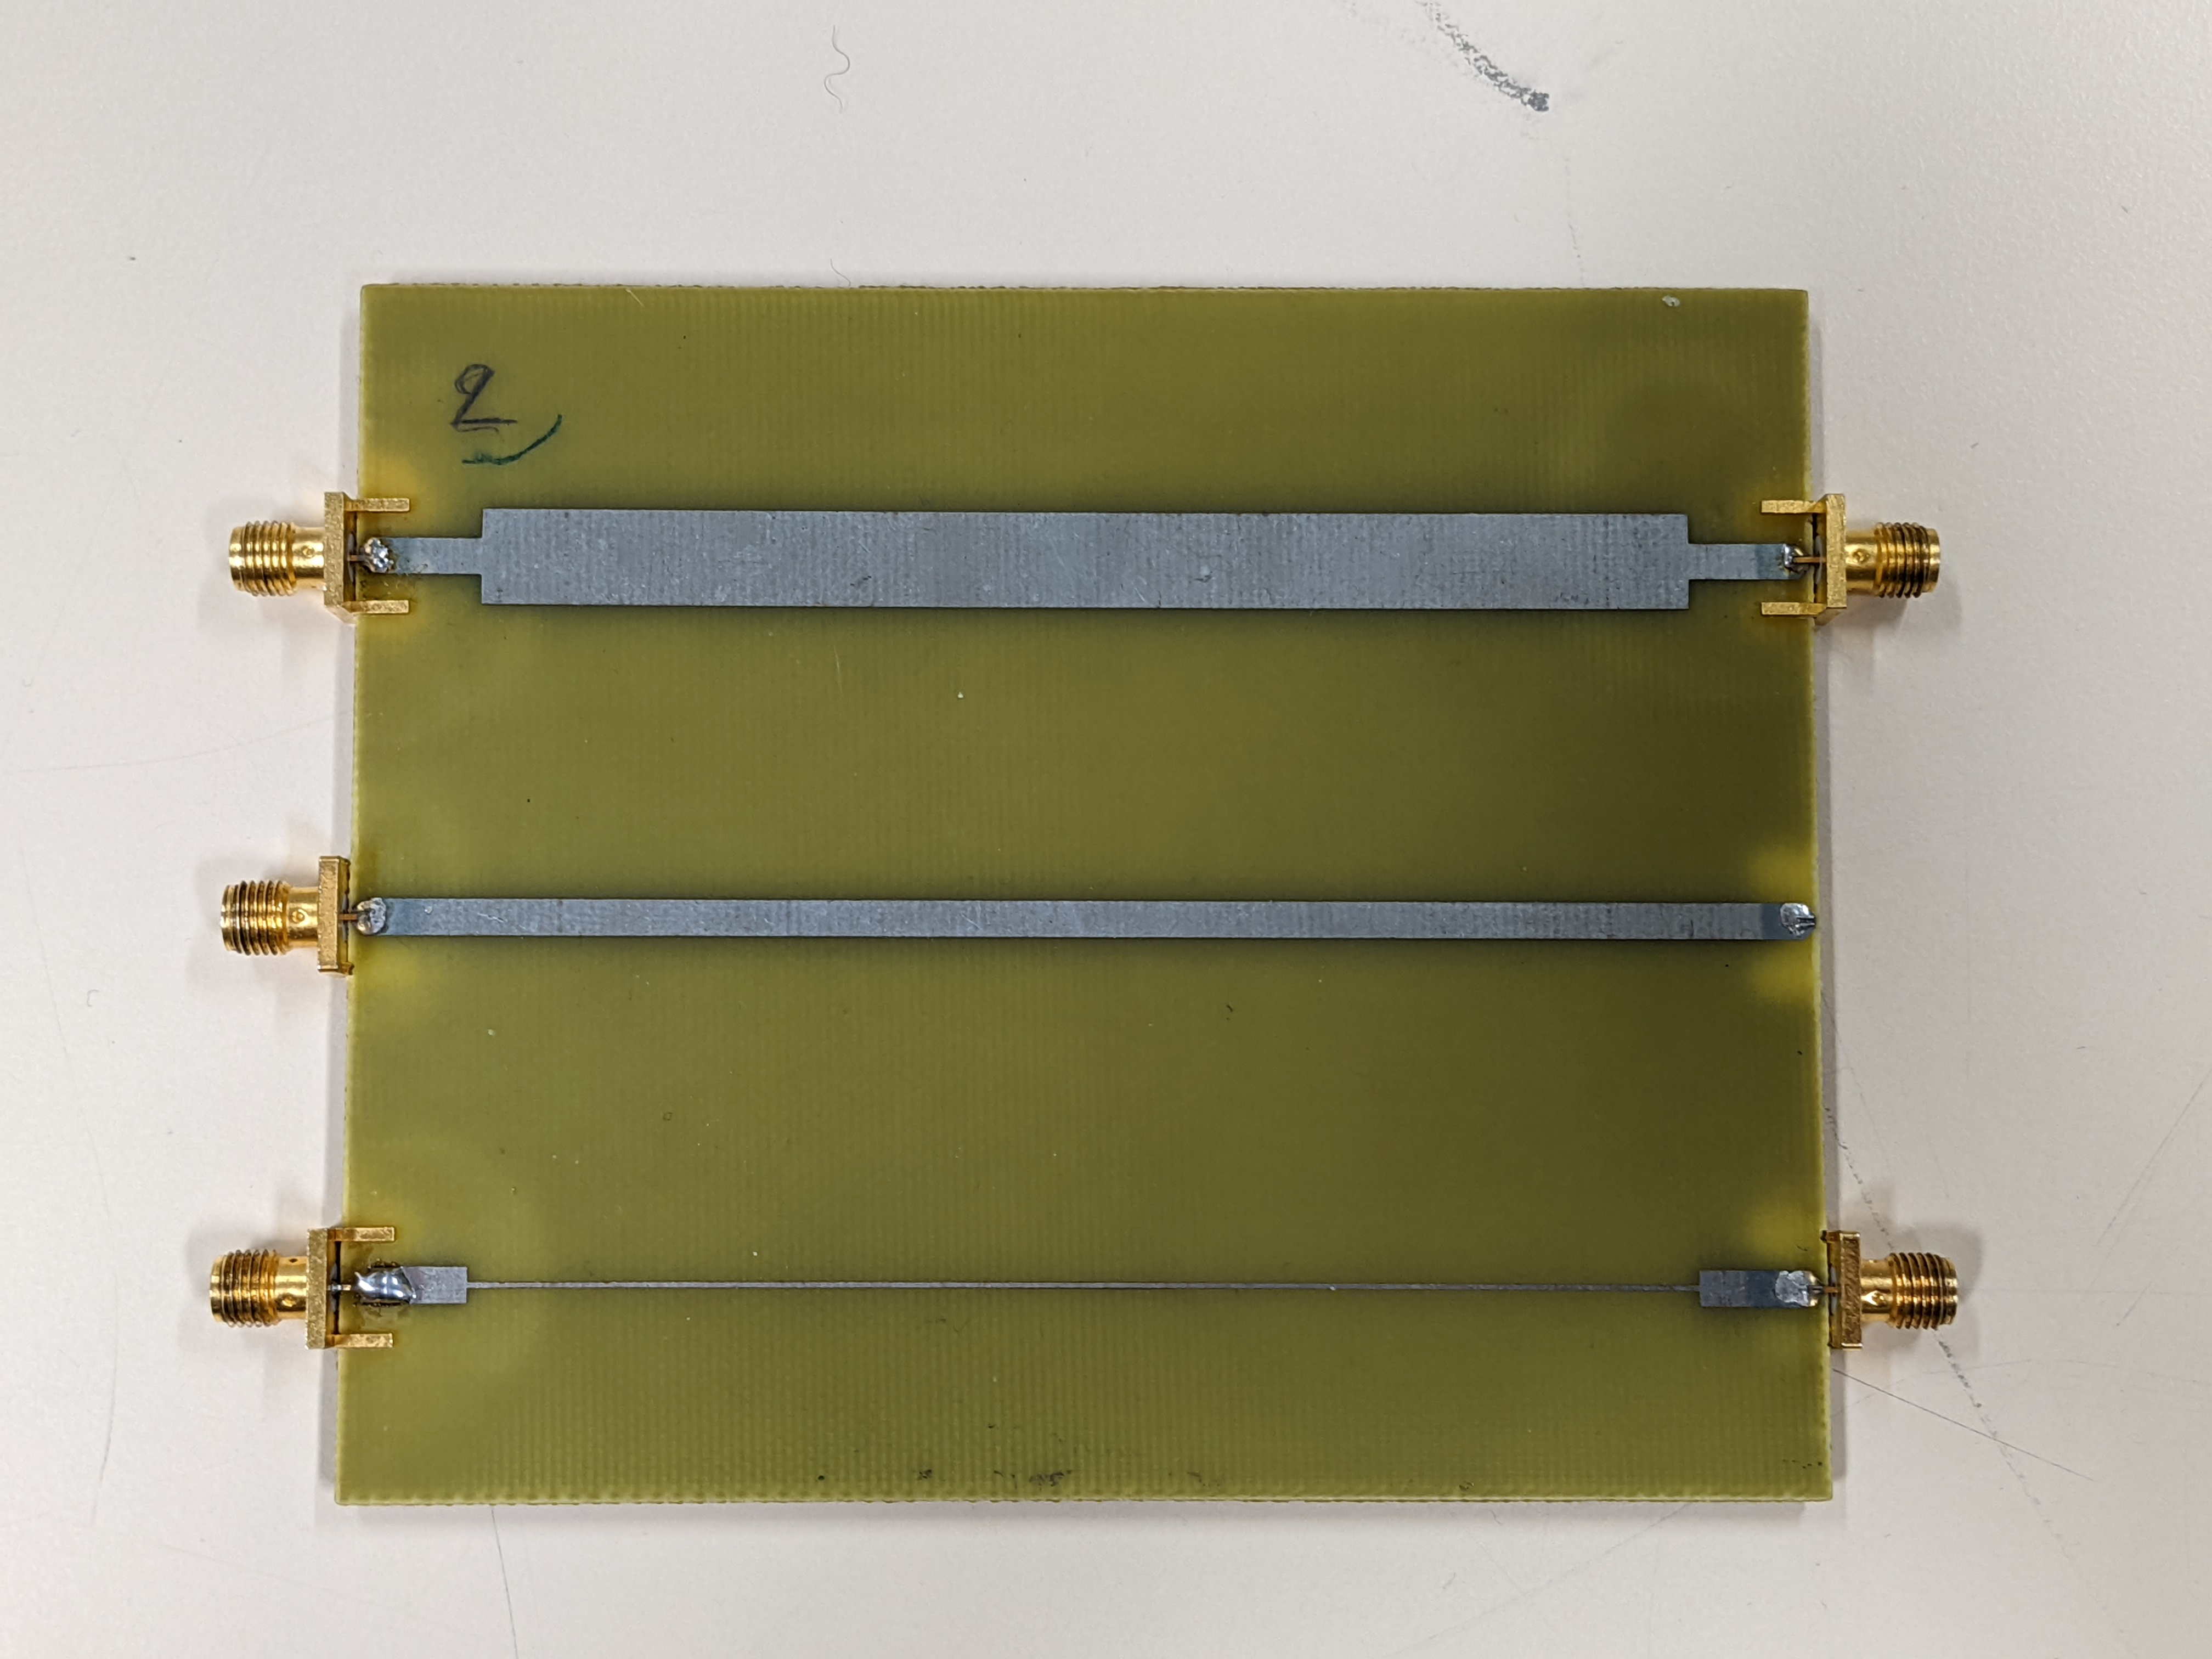
\includegraphics[scale=0.07]{photo/ligne et filtre/plaque_caract_epoxy.jpg}
\begin{center}
	Annexe 1 : Photographies de plaques avec des lignes de caractérisation (à gauche plaque en verre téflon et à gauche en verre epoxy FR4)
\end{center}


\end{document}
